% Format teze zasnovan je na paketu memoir
% http://tug.ctan.org/macros/latex/contrib/memoir/memman.pdf ili
% http://texdoc.net/texmf-dist/doc/latex/memoir/memman.pdf
% 
% Prilikom zadavanja klase memoir, navedenim opcijama se podešava 
% veličina slova (12pt) i jednostrano štampanje (oneside).
% Ove parametre možete menjati samo ako pravite nezvanične verzije
% mastera za privatnu upotrebu (na primer, u b5 varijanti ima smisla 
% smanjiti 
\documentclass[12pt,oneside]{memoir} 

% Paket koji definiše sve specifičnosti master rada Matematičkog fakulteta
\usepackage[latinica,biblatex]{matfmaster} 
%
% Podrazumevano pismo je ćirilica.
%   Ako koristite pdflatex, a ne xetex, sav latinički tekst na srpskom jeziku
%   treba biti okružen sa \lat{...} ili \begin{latinica}...\end{latinica}.
%
% Opicija [latinica]:
%   ako želite da pišete latiniciom, dodajte opciju "latinica" tj.
%   prethodni paket uključite pomoću: \usepackage[latinica]{matfmaster}.
%   Ako koristite pdflatex, a ne xetex, sav ćirilički tekst treba biti
%   okružen sa \cir{...} ili \begin{cirilica}...\end{cirilica}.
%
% Opcija [biblatex]:
%   ako želite da koristite reference na više jezika i umesto paketa
%   bibtex da koristite BibLaTeX/Biber, dodajte opciju "biblatex" tj.
%   prethodni paket uključite pomoću: \usepackage[biblatex]{matfmaster}
%
% Opcija [b5paper]:
%   ako želite da napravite verziju teze u manjem (b5) formatu, navedite
%   opciju "b5paper", tj. prethodni paket uključite pomoću: 
%   \usepackage[b5paper]{matfmaster}. Tada ima smisla razmisliti o promeni
%   veličine slova (izmenom opcije 12pt na 11pt u \documentclass{memoir}).
%
% Naravno, opcije je moguće kombinovati.
% Npr. \usepackage[b5paper,biblatex]{matfmaster}

% Pomoćni paket koji generiše nasumičan tekst u kojem se javljaju sva slova
% azbuke (nema potrebe koristiti ovo u pravim disertacijama)
\usepackage[latinica]{pangrami}
\usepackage{listings}
\usepackage{xcolor}
 
 \hypersetup{
    colorlinks=true,
    linkcolor=blue,
    filecolor=magenta,      
    urlcolor=cyan,
    citecolor=blue
}
 
\definecolor{codegreen}{rgb}{0,0.6,0}
\definecolor{codegray}{rgb}{0.5,0.5,0.5}
\definecolor{codepurple}{rgb}{0.58,0,0.82}
\definecolor{backcolour}{rgb}{0.95,0.95,0.92}
 
\lstdefinestyle{mystyle}{
    backgroundcolor=\color{backcolour},   
    commentstyle=\color{codegreen},
    keywordstyle=\color{magenta},
    numberstyle=\tiny\color{codegray},
    stringstyle=\color{codepurple},
    basicstyle=\ttfamily\footnotesize,
    breakatwhitespace=false,         
    breaklines=true,                 
    captionpos=b,                    
    keepspaces=true,                 
    numbers=left,                    
    numbersep=5pt,                  
    showspaces=false,                
    showstringspaces=false,
    showtabs=false,                  
    tabsize=2
}

\lstset{style=mystyle}

% \newcommand{\source}[1]{\caption*{\scriptsize{Izvor: {#1}}}} % Source for pictures

% Datoteka sa literaturom u BibTex tj. BibLaTeX/Biber formatu
\bib{matfmaster-primer}

% Ime kandidata na srpskom jeziku (u odabranom pismu)
\autor{Milena Dukanac}
% Naslov teze na srpskom jeziku (u odabranom pismu)
\naslov{Jezik Elixir sa primenom u sekvencioniranju genoma}
% Godina u kojoj je teza predana komisiji
\godina{2019}
% Ime i afilijacija mentora (u odabranom pismu)
\mentor{dr Milena \textsc{Vujošević Janičić}, docent\\ Univerzitet u Beogradu, Matematički fakultet}
% Ime i afilijacija prvog člana komisije (u odabranom pismu)
\komisijaA{dr Jovana \textsc{Kovačević}, docent\\ Univerzitet u Beogradu, Matematički fakultet}
% Ime i afilijacija drugog člana komisije (u odabranom pismu)
\komisijaB{dr Vesna \textsc{Marinković}, docent\\ Univerzitet u Beogradu, Matematički fakultet}
% Ime i afilijacija trećeg člana komisije (opciono)
% \komisijaC{}
% Ime i afilijacija četvrtog člana komisije (opciono)
% \komisijaD{}
% Datum odbrane (odkomentarisati narednu liniju i upisati datum odbrane ako je poznat)
% \datumodbrane{}

% Apstrakt na srpskom jeziku (u odabranom pismu)
\apstr{%
%\pangrami
}

% Ključne reči na srpskom jeziku (u odabranom pismu)
\kljucnereci{}

\begin{document}
% ==============================================================================
% Uvodni deo teze
\frontmatter
% ==============================================================================
% Naslovna strana
\naslovna
% Strana sa podacima o mentoru i članovima komisije
\komisija
% Strana sa posvetom (u odabranom pismu)
\posveta{Mami i tati}
% Strana sa podacima o disertaciji na srpskom jeziku
\apstrakt
% Sadržaj teze
\tableofcontents*

% ==============================================================================
% Glavni deo teze
\mainmatter
% ==============================================================================

% ------------------------------------------------------------------------------
\chapter{Elixir} %A bio je Uvod
% ------------------------------------------------------------------------------
%\pangrami

Elixir je funkcionalan programski jezik nastao 2011. godine. Njegovim tvorcem se smatra Hosé Valim (engl. \textit{José Valim}). Elixir je dizajniran za izgradnju skalabilnih i lako održivih aplikacija. Poseduje jednostavnu i modernu sintaksu. Zbog svoje funkcionalne prirode, izuzetnog rada u distrubiranim sistemima i tolerancije na greške koja je na jako visokom nivou, u Elixir-u je rađeno mnogo zanimljivih projekata u vezi sa robotikom. Takođe se uspešno koristi u razvoju veba i u domenu softvera za uređaje sa ugrađenim računarom (engl. \textit{embedded sotfware}).

\newpage

\section{Jezici sa najviše uticaja}
Na nastanak Elixir-a je uticao programski jezik \textbf{Erlang}. 
\begin{comment}Elixir radi uz podršku virtualne mašine ovog jezika koja je karakteristična po minimalnom kašnjenju i zavidnoj toleranciji na greške. 
\end{comment}
Pri njegovom kreiranju značajnu ulogu u smislu sintakse imao je programski jezik \textbf{Ruby}, a iz jezika kao što su \textbf{Python, Haskell} i \textbf{Clojure} je preuzeo mnoge koncepte. Dijagram uticaja ovih jezika na Elixir, kao i vreme nastanka svakog od njih može se videti na slici \ref{fig:02}: 
\begin{comment}
U Elixir-u ne postoje objekti i klase, već se sve zasniva na funkcijama i rekurziji. (izmeni) 
\end{comment}

\begin{figure}[!ht]
  \centering
  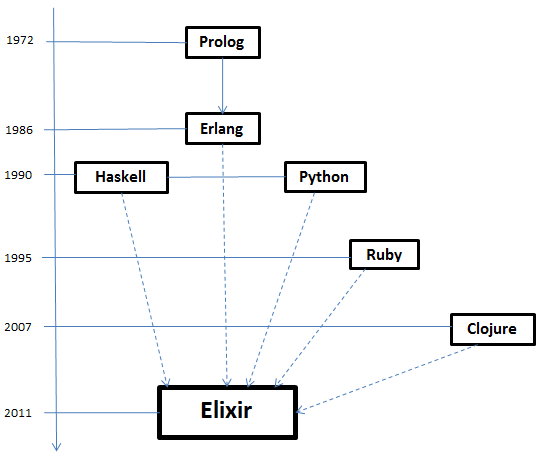
\includegraphics[width=\textwidth]{dijagram_uticaja_jezika.PNG}
  \caption{Dijagram uticaja ostalih jezika na Elixir}
  \label{fig:02}
\end{figure}

\newpage

\subsection{Lisp}
\textbf{Lisp} je drugi najstariji viši programski jezik koji se i danas veoma koristi. Imao je uticaj na programski jezik Erlang, pa je samim tim uticao i na Elixir. Lisp je projektovao \textbf{Džon Makarti} 1958. godine, a prvi put je implementiran od strane \textbf{Stiva Rasela} na IBM 704 računaru. Rasel je pročitao Makartijev rad i zaključio da izračunavanje u Lispu može da se implementira na mašinskom jeziku. Rezultat toga je bio  interpretator koji je mogao da pokreće Lisp programe, ali i da računa vrednosti Lisp izraza. Lisp je zasnovan na matematičkoj teoriji rekurzivnih funkcija (u kojoj se funkcija pojavljuje u sopstvenoj definiciji), a Lisp program je funkcija koja se primenjuje na podatke. On koristi vrlo jednostavnu notaciju u kojoj se operacije i njihovi operandi prikazuju u zagradi. Na primer, $(+ a ( * b c))$ predstavlja $a + b * c$. Iako se čini neugodna, ova notacija dobro funkcioniše na računarima. Ime LISP je nastalo od \textit{"\textbf{LIS}t \textbf{P}rocessor"}, a povezane liste su jedan od glavnih tipova podataka. Danas postoji veliki broj dijalekata Lisp-a, a najpoznatiji među njima su \textbf{Common Lisp} i \textbf{Scheme}. Osnova Lisp-a je funkcionalno programiranje, ali se Lisp zbog raznih drugih svojstava smatra multiparadigmatskim programskim jezikom.

\subsection{Prolog}
\textbf{Prolog} (engl. \textit{\textbf{PRO}gramming in \textbf{LOG}ic}) je deklarativan programski jezik namenjen rešavanju zadataka simboličke prirode. On bio osnova za Erlang, te je imao indirektan uticaj i na Elixir. Prolog se temelji na teorijskom modelu logike prvog reda. Početkom 1970-ih godina \textbf{Alain Kolmerauer} (engl. \textit{Alain Colmerauer}) i \textbf{Filipe Rousel} (engl. \textit{Philippe Roussel}) na Univerzitetu u Marselju (engl. \textit{University of Aix-Marseille}), zajedno sa \textbf{Robertom Kovalskim} (engl. \textit{Robert Kowalski}) sa Departmana veštačke inteligencije (engl. \textit{Department of Artifical Intelligence}) na Univerzitetu u Edinburgu (engl. \textit{University of Edinburgh}), razvili su osnovni dizajn jezika Prolog.

\newpage

\subsection{Erlang}
Firma Erikson je 1981. godine oformila novu laboratoriju \textbf{Erikson CSLab} (eng. \textit{The Ericsson CSLab}) sa ciljem da predlaže i stvara nove arhitekture, koncepte i strukture za buduće softverske sisteme. Jedan od projekata nove laboratorije  je bio eksperimentisanje sa dodavanjem konkurentnih procesa u programski jezik Prolog i on predstavlja začetak novog programskog jezika. Taj programski jezik je 1987. godine nazvan \textbf{Erlang}. Ime je nastalo zahvaljujući inicijativi zaposlenih koji su radili na telefonskim prekidačima, a  za koje je jezik dizajniran. Naime, oni su predložili da jezik nosi ime Erlang u čast danskom matematičaru i inženjeru Agneru Krarupu Erlangu (engl. \textit{Agner Krarup Erlang}), a što je ujedno odgovaralo i skraćenici od  "\textbf{Er}icsson \textbf{Lang}uage".  Erlang se mogao posmatrati kao dijalekt Prologa sve do 1990. godine. Od tada, on ima svoju sintaksu i postoji kao potpuno samostalan programski
jezik. Nakon mnogo godina rada nastajale su sve brže, bolje i stabilnije verzije jezika, kao i \textbf{standardna biblioteka OTP} (eng. \textit{The Open Telecom Platform}) (referenca). Erlang i OTP su postali deo slobodnog softvera (eng. \textit{open source software}) u decembru 1998. godine i mogu se slobodno preuzeti sa zvaničnog sajta jezika Erlang. Veliki broj kompanija danas koristi Erlang u razvoju svojih softverskih rešenja. Neke od
njih su: Erikson (engl. \textit{Ericsson}), Motorola, Votsap (eng. \textit{WhatsApp}), Jahu (eng. \textit{Yahoo!}),
Fejsbuk (eng. \textit{Facebook}) (referenca).

\textbf{Erlang} je funkcionalan, deklarativan i konkurentan programski jezik. Na planu konkurentnosti je
svojevrstan primer. Programski jezik Lisp je prvi predstavio funkcionalnu paradigmu i kao takav je imao veliki uticaj na Erlang. Neki od koncepata i osobina koje je nasledio od Lisp-a su koncept rekurzije, \textit{list comprehension} - sintaktička konstrukcija za kreiranje liste zasnovane na postojećim listama, koja sledi formu matematičke notacije \textit{set-builder} za razliku od upotrebe funkcija mapiranja i filtera. Na početku je Erlang stvaran kao dodatak na Prolog, vremenom je prerastao
u dijalekt Prologa, a kasnije je zbog svoje kompleksnosti i sveobuhvatnosti evoluirao u potpuno novi programski jezik. Sintaksa jezika Erlang u velikoj meri podseća na sintaksu jezika Prolog (na primer, promenljive moraju počinjati velikim slovom, svaka funkcionalna celina se završava tačkom). Oba jezika u velikoj meri koriste poklapanje obrazaca (eng. \textit{pattern matching}).

Sa druge strane, Erlang je uticao na nastanak programskog jezika Elixir. Uz izmenjenu Erlangovu sintaksu i dopunjenu Erlangovu standardnu biblioteku, Elixir uživa široku popularnost.
     
\begin{comment} U funkcionalnom programiranju, funkcije se primenjuju na argumente i vrednosti. Vraćene vrednosti se koriste kao argumenti za druge funkcije. Funkcionalno programiranje je suprotno proceduralnom programiranju, gde se koriste naredbe koje menjaju okruženje programa na neki način, kao što je pripisivanje vrednosti promenljivim. U funkcionalnom programiranju, te promene okruženja se minimizuju korišćenjem vrednosti koje vraća pozvana funkcija kao direktan ulaz u drugu funkciju, bez upotrebe pripisivanja naredbi.\\
\end{comment}

\subsection{Python}
\textbf{Python} je interpretirani jezik opšte namene čiji tvorac je Gido van Rosum (engl. \textit{Guido van Rossum}). Krajem 1980-ih je koncipiran kao naslednik jezika \textbf{ABC}, a prvi put je objavljen 1991. godine. Filozofija dizajna jezika Python naglašava čitljivost koda pridavajući veliki značaj razmaku. Njegove jezičke konstrukcije i objektno-orijentisani pristup imaju za cilj da pomognu programerima da napišu jasan i logičan kod za male i velike projekte. Python je takođe dinamički tipiziran jezik i poseduje sistem za prikupljanje smeća (\textit{garbage collector}). Podržava više paradigmi programiranja uključujući proceduralno, objektno-orijentisano i funkcionalno programiranje. Python interpreteri su dostupni za mnoge operativne sisteme. Globalana zajednica programera razvija i održava referentnu implementaciju otvorenog koda \textbf{CPython}. Neprofitna organizacija \textit{The Python Software Foundation} upravlja i usmerava resursima za razvoj jezika Python i CPython. Jedna od osobina koje je Elixir nasledio od Python-a je podrška za dokumentaciju u vidu dokumentacionih stringova (engl. \textit{docstrings}) koji omogućavaju povezivanje dokumentacije sa modulima, funkcijama, klasama, metodama.

\subsection{Haskell}
\textbf{Haskell} je čisto funkcionalni jezik koji je statički tipiziran i prilično različit od većine ostalih programskih jezika. Nazvan je po Haskel Bruks Kariju(engl. \textit{Haskell Brooks Curry}), čiji rad u oblasti matematičke logike služi kao osnova za sve funkcionalne jezike. Haskell je zasnovan na lambda računu, pa se stoga lambda koristi kao logo jezika. Nudi kratak, jasan i održiv kod, mali procenat grešaka i veliku pouzdanost. Stoga je pogodan za pisanje velikih softverskih sistema, jer njihovo održavanje čini lakšim i jeftinijim. Jedna od karakteristika koje je Elixir preuzeo od ovog jezika je lenjo izračunavanje.

\subsection{Ruby}
\textbf{Ruby} je dinamički tipiziran programski jezik otvorenog koda nastao 1995. godine. Fokus kod ovog programskog jezika je na jednostavnosti i produktivnosti. Ruby ima elegantnu sintaksu koja je prirodna za čitanje i lako pisanje.
Ruby je takođe i interpretirani programski jezik, što znači da se izvorni kod prevodi u kod razumljiv kompjuteru prilikom svakog izvršavanja programa. Interpretirani programski jezici su sporiji od kompajliranih, ali su fleksibilniji i potrebno je kraće vreme za izradu programa.
Međutim, sve više iskusnih Ruby programera se okreće Elixir-u. Zapravo, Elixir je prvi jezik nakon Ruby-ja koji zaista brine o lepoti koda i korisničkom iskustvu vezanom za jezik, biblioteke i ekosistem. Na slici \ref{fig:0} su prikazane osobine Ruby-ja koje se direktno preslikavaju u osobine Elixir-a:

\begin{figure}[!ht]
  \centering
  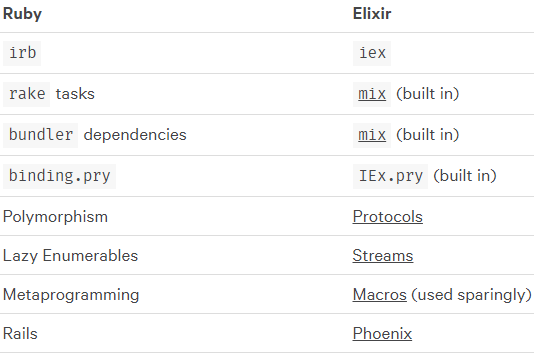
\includegraphics[width=0.8\textwidth]{ruby.PNG}
  \caption{Osobine nasleđene od jezika Ruby}
  \label{fig:0}
\end{figure}

Takođe, na slici \ref{fig:01} se može videti i primer koda napisan u oba jezika:

\begin{figure}[!ht]
  \centering
  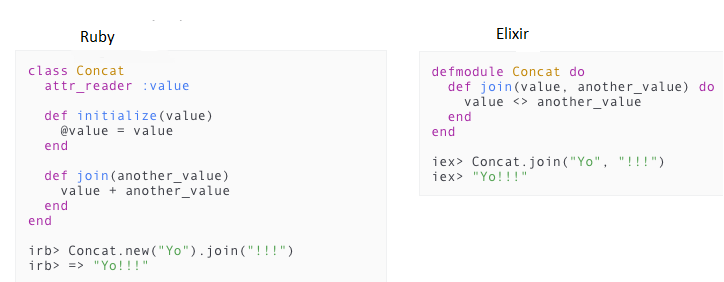
\includegraphics[width=\textwidth,height=6.5cm]{rubyVSelixir.png}
  \caption{Sintaksa jezika Ruby i Elixir}
  \label{fig:01}
\end{figure}

\subsection{Clojure}
\textbf{Clojure} je dinamički tipiziran programski jezik opšte namene nastao 2007. godine. Njegov tvorac je Rič Hiki (engl. \textit{Rich Hickey}). Clojure kombinuje pristupačnost i interaktivni razvoj skriptnog jezika sa efikasnom i robusnom infrastrukturom za višenitno programiranje. On je kompajlirani jezik, ali je i dalje potpuno dinamički tipiziran - svaka funkcija koju podržava Clojure je podržana u toku izvršavanja. Predstavlja dijalekt jezika Lisp i deli njegovu filozofiju \textit{code-as-data} (program je funkcija koja se izvršava nad podacima) i moćan makro sistem. Clojure je pretežno funkcionalni programski jezik i sadrži bogat skup nepromenljivih i postojanih struktura podataka. Elixir je nasledio neke od najboljih Clojure karakteristika - efikasne, nepromenljive strukture podataka (imutabilnost), opcionalno lenjo izračunavanje, protokole.
\newpage

\section{Osnovne karakteristike}

Tokom 2010. godine Hosé Valim, u to vreme zaposlen na poziciji programera u kompaniji \textit{Platformatec}, radio je na poboljšanju performansi okruženja
\textit{Ruby on Rails} na višejezgarnim sistemima.(referenca) Shvatio je da Ruby nije bio dovoljno dobro dizajniran da reši problem konkurentnosti, pa je započeo istraživanje drugih tehnologija koje bi bile prihvatljivije. Tako je otkrio Erlang i upravo ga je interesovanje prema virtuelnoj mašini jezika Erlang podstaklo da započne pisanje jezika Elixir. Uticaj projekta na kome je do tada radio odrazio se na to da Elixir ima sintaksu koja je nalik na sintaksu jezika Ruby. Ovaj jezik se pokazao veoma dobro pri upravljanju
milionima simultanih konekcija: u 2015. je zabeleženo upravljanje nad 2 miliona \textit{WebSocket} konekcija, dok je u 2017. za skalirani Elixir zabeležena obrada 5 miliona istovremenih korisnika. Elixir se danas koristi u velikim kompanijama, kao što su \textit{Discord}  i \textit{Pinterest}.\\

Elixir je dinamički tipiziran, funkcionalni programski jezik koji se pokreće na vituelnoj mašini jezika Erlang, pa samim tim i nasleđuje pogodna svojstva koje dolaze sa ovim okruženjem kao što su \textbf{konkurentnost} i \textbf{tolerisanje grešaka}. Iz tačke gledišta olakšavanja svakodnevnog razvoja sofvera, mnogi koncepti su falili ekosistemu jezika Erlang. Neki od njih su \textbf{metaprogramiranje} - tehnika kojom programi imaju mogućnost da druge programe posmatraju kao svoje podatke i na taj način čitaju, pa
čak i modifikuju njihov, a samim tim i svoj kod u vreme izvršavanja, \textbf{polimorfizam}, \textbf{makroi}, \textbf{podrška za alate}. Upravo navedene koncepte je  Elixir nadomestio. Cilj ovog rada je da čitaoca bliže upozna sa osnovnim osobinama, funkcionalnostima i specifičnostima ovog jezika,  kao i da kroz primere pokuša da približi programerske prakse korišćene u ovom jeziku.

U ovom delu će biti opisane osobine jezika Elixir, osnove njegove sintakse, semantike, kao i podrška za osnovne koncepte funkcionalnih jezika poput poklapanja obrazaca (eng. \textit{Pattern matching}) i imutabilnosti podataka.

Pre nego što započnemo priču o tipovima, treba pomenuti \textbf{Kernel}. To je podrazumevano okruženje koje se koristi u Elixir-u. Ono sadrži primitive jezika kao što su: aritmetičke operacije, rukovanje procesima i tipovima, makroe za definisanje novih funkcionalnosti (funkcija, modula...), provere guard-ova - predefinisanog skupa funkcija i makroa koji proširuju
mogućnost pattern matching-a, itd.

\section{Osnovni tipovi podataka}

Elixir ima svoje ugrađene (primitivne) tipove. To su: 
\begin{enumerate}
    \item {Atomi}
    \item {Celi brojevi}
    \item {Brojevi u pokretnom zarezu}
    \item {Portovi}
    \item {Ugrađene torke}
    \item {Liste}
    \item {Mape}
    \item {Funkcije}
    \item {Niske bitova}
    \item {Reference}
\end{enumerate}

Svaki od ovih tipova, osim poslednja dva, ima odgovarajuće module koji sadrže funkcije koje se koriste za operacije nad tim tipom. Oni predstavljaju omotač oko primitivnog tipa koji nam omogućava korišćenje dodatnih funkcionalnosti nad njim. U nastavku će biti opisani neki od osnovnih tipova.\\

\subsubsection{Atomi}
Atomi su konstante ili simboli, pri čemu njihovo ime predstavlja njihovu vrednost. Počinju dvotačkom (:) i mogu sadržati slova, cifre, simbole \_, @. Mogu se završavati sa ! i ?. Atomi se mogu naći svuda u Elixir-u. Oni su ključevi za listu ključnih reči, koji se često koriste da označe uspeh ili grešku, npr. :ok i mnogi drugi.\\

\subsubsection{Celi brojevi}
Celi brojevi su slični kao i u većini ostalih jezika i mogu biti dekadni, heksadekadni, oktalni i binarni. Karakter \_ se može koristiti za odvajanje blokova cifara. Veoma značajna stvar je da ne postoji fiksna veličina za čuvanje celih brojeva u memoriji, već interna reprezentacija raste kako bi broj mogao biti smešten u celosti.\\

\subsubsection{Brojevi u pokretnom zarezu}
Brojevi u pokretnom zarezu se u memoriji zapisuju po standardu \textit{IEEE 754}, a za zapisivanje konstanti ovog tipa koristi se tačka između najmanje 2 cifre. Takođe je moguće koristiti notaciju koja obuhvata navođenje eksponenata.\\

\begin{comment}
\subsubsection{Procesi}
U Elixir-u se sav kod pokreće unutar procesa. Procesi su izolovani jedni od drugih, spajaju se jedan sa drugima i komuniciraju putem slanja poruka. Procesi nisu samo osnova za konkurentnost u Elixir-u, već i sredstva za izgradnju distribuiranih i tolerantnih programa.
Procese Elixir-a ne treba mešati sa procesima operativnog sistema. Procesi Elixira su izuzetno lagani u smislu memorije i CPU-a (čak i u poređenju sa nitima koji se koriste u mnogim drugim programskim jezicima). Zbog toga nije neuobičajeno da se istovremeno odvijaju desetine ili čak stotine hiljada procesa.\\
\end{comment}

\begin{comment}
\subsubsection{Portovi i reference}
Portovi ukazuju na spoljne resurse koje omogućavaju interakciju sa spoljnim svetom.\\

Reference su jedinstvene vrednosti u globalnom kontekstu izvršavanja programa koje se kreiraju pozivom \textit{make\_ref} funkcije.\\
\end{comment}

\subsubsection{Liste}
Liste se čuvaju u memoriji kao povezane liste, što znači da svaki element u listi čuva svoju vrednost i ukazuje na sledeći element sve dok se ne dostigne kraj liste. To znači da je pristup proizvoljnom elementu liste kao i određivanje družine liste linearna operacija, jer je potrebno da prođemo celu listu da bismo odredili njenu dužinu. Slično, performanse spajanja dve liste zavise od dužine one koja se nalazi sa leve strane. 

Elixir koristi uglaste zagrade $([])$ da označi listu vrednosti. Vredosti mogu biti bilo kog tipa, a primer liste sa vrednostima različitih tipova prikazan je na listingu \ref{lst:prvi}:

\lstinputlisting[language=erlang,label={lst:prvi},caption=Primer liste,captionpos=b]{prvi.ex}

\newpage

Nadovezivanje ili oduzimanje 2 liste korišćenjem operatora $++/2$ i $--/2$ prikazano je na listingu \ref{lst:drugi}:

\lstinputlisting[language=erlang,label={lst:drugi},caption=Nadovezivanje i oduzimanje dve liste,captionpos=b]{drugi.ex}

Operatori liste nikada ne menjaju postojeću listu. Rezultat povezivanja listi ili uklanjanja elemenata iz liste je uvek nova lista, jer su strukture podataka u Elixir-u nepromenljive. Jedna od prednosti nepromenljivosti je jasniji kod. Omogućeno je slobodno prosleđivanje podatka sa garancijom da neće biti izmenjeni u memoriji - samo transformisani.

Lista može biti prazna ili se može sastojati od \textbf{glave} i \textbf{repa}. Glava je prvi element liste, a rep je ostatak liste. Oni se mogu izdvojiti pomoću funkcija \textit{hd/1} i \textit{tl/1}. Dodeljivanje liste promenljivoj, dohvatanje njene glave i repa prikazano je na listingu \ref{lst:treci}:

\lstinputlisting[language=erlang,label={lst:treci},caption=Izdvajanje glave i repa liste,captionpos=b]{treci.ex}

Ako pokušamo da izdvojimo glavu ili rep prazne liste, dobićemo grešku.

Prilikom kreiranja liste može se desiti da je rezultat lista vredosti pod jednostrukim navodnicima. Primer koda koji ilustruje ovo može se videti na listingu \ref{lst:cetvrti}:

\lstinputlisting[language=erlang,label={lst:cetvrti},caption=Lista vrednosti pod jednostrukim navodnicima,captionpos=b]{cetvrti.ex}

Kada Elixir vidi listu \textit{ASCII} brojeva za štampanje, ispisaće je kao \textit{charlist}-u (doslovno listu znakova). Charlist-e su uobičajene kada se povezuju sa postojećim Erlang kodom. Preuzimanje informacija o vrednosti za koju nismo sigurni kog je tipa može se izvršiti pomoću funkcije \textit{i/1} i može se videti na listingu \ref{lst:peti}:

\lstinputlisting[language=erlang,label={lst:peti},caption=Preuzimanje informacija o tipu vrednosti,captionpos=b]{peti.ex}

Treba imati na umu da reprezentacije sa jednostrukim i dvostrukim navodnicima u Elixir-u nisu ekvivalentne i da predstavljaju različite tipove. Primer možemo videti na listingu \ref{lst:sesti}:

\lstinputlisting[language=erlang,label={lst:sesti},caption=Dva različita tipa,captionpos=b]{sesti.ex}

\subsection{Torke}

Torke se u Elixir-u definišu pomoću vitičastih zagrada $\{\}$. Kao i liste, mogu sadržati vrednosti bilo kog tipa. Primer torke sa vrednostima različitih tipova i određivanjem njene dužine prikazan je na listingu \ref{lst:sedmi}:

\lstinputlisting[language=erlang,label={lst:sedmi},caption=Primer torke i određivanje njene dužine,captionpos=b]{sedmi.ex}

Torke su strukture fiksne dužine koje bi trebalo da sadrže svega nekoliko elemenata koji su zapisani u memoriji jedan za drugim. To znači da se pristup elementu torke ili određivanje dužine torke izvršava u konstantnom vremenu. Razlika u odnosu na liste je u semantici upotrebe. Liste se koriste kada se manipuliše kolekcijom, dok se torke, zbog brzine pristupa njihovim elementima, uglavnom koriste za smeštanje povratne vrednosti funkcije. Indeksi torke počinju od nule, a primer se može videti na listingu \ref{lst:osmi}:

\lstinputlisting[language=erlang,label={lst:osmi},caption=Izdvajanje elementa torke sa indeksom 1,captionpos=b]{osmi.ex}

Takođe je moguće umetnuti novi element na odredjeno mesto u torki pomoću funkcije $put\_elem/3$. Primer koda koji ilustruje upotrebu ove funkcije prikazan je na listingu \ref{lst:deveti}:

\lstinputlisting[language=erlang,label={lst:deveti},caption=Umetanje novog elementa u torku,captionpos=b]{deveti.ex}

Treba obratiti pažnju da je funkcija $put\_elem/3$ vratila novu torku. Originalna torka smeštena u promenljivoj \textit{tuple} nije izmenjena. Kao i liste, torke su takođe nepromenljive. Svaka operacija nad torkom vraća novu torku i nikada ne menja postojeću. Ova operacija, kao i operacija ažuriranja torke je skupa, jer zahteva kreiranje nove torke u memoriji. Ovo se odnosi samo na samu torku, a ne na njen sadržaj. Na primer, prilikom ažuriranja torke, svi unosi se dele između stare i nove torke, osim unosa koji je zamenjen. Drugim rečima, torke i liste u Elixir-u mogu da dele svoj sadržaj. Ovo smanjuje količinu memorije koju jezik treba da zauzme i moguće je samo zahvaljujući nepromenljivoj semantici jezika.

Ove karakteristike performansi diktiraju upotrebu struktura podataka. Kao što je već pomenuto, jedan od uobičajenih slučajeva korišćenja torki je prilikom vraćanja dodatnih vrednosti iz funkcije. \textit{File.read/1} je funkcija koja se može koristiti za čitanje sadržaja datoteke. Ona vraća torku, što se može videti na listingu \ref{lst:deseti}:

\lstinputlisting[language=erlang,label={lst:deseti},caption=Primer korišćenja funkcije \textit{File.read/1},captionpos=b]{deseti.ex}

Ako putanja do fajla postoji, povratna vrednost funkcije je torka sa prvim elementom koji je atom :ok i drugim elementom koji je sadržaj datog fajla. U suprotnom, povratna vrednost funkcije će biti torka gde je prvi element atom :error, a drugi element opis greške.

\subsection{Liste ključnih reči i mape}
Elixir podržava asocijativne strukture podataka. Asocijativne strukture podataka su one koje su u stanju da pridruže određenu vrednost ili više vrednosti ključu. Dve glavne strukture među njima su \textbf{liste ključnih reči} i \textbf{mape}.

\subsubsection{Liste ključnih reči}
U mnogim funkcionalnim programskim jezicima, uobičajeno je da se koristi lista dvočlanih torki za predstavljanje strukture podataka ključ - vrednost. Lista torki gde je prvi element torke atom (tj. ključ) u Elixir-u se naziva \textbf{lista ključnih reči}. Elixir podržava posebnu sintaksu za definisanje takvih lista: $[key: value]$. Zapravo, liste ključnih reči mapiraju liste torki. Primer ovakvog mapiranja prikazan je na listingu \ref{lst:11}:


\lstinputlisting[language=erlang,label={lst:11},caption=Primer liste ključnih reči,captionpos=b]{11.ex}

 Kako su liste ključnih reči liste, nad njima možemo primenjivati sve operacije dostupne nad listama. Na primer, korišćenjem operatora ++ može se izvršiti dodavanje nove vrednosti listi ključnih reči. Primer koda koji ilustruje ovo dodavanje dat je na listingu \ref{lst:12}:

\lstinputlisting[language=erlang,label={lst:12},caption=Dodavanje nove vrednosti listi ključnih reči,captionpos=b]{12.ex}

Elementima liste ključnih reči se pristupa na način prikazan na listingu \ref{lst:13}:

\lstinputlisting[language=erlang,label={lst:13},caption=Pristup elementu liste ključnih reči,captionpos=b]{13.ex}

Liste ključnih reči su važne, jer imaju tri posebne karakteristike:
\begin{enumerate}
\item{Ključevi moraju biti atomi.}
\item{Ključevi su uredjeni, onako kako je navedeno od strane programera.}
\item{Ključevi se mogu ponavljati.}
\end{enumerate}

 Elixir obezbeđuje modul koji omogućava manipulisanje listama ključnih reči. Liste ključnih reči su jednostavno liste, i kao takve pružaju iste karakteristike linearnih performansi kao i liste. Što je lista duža, više vrmena će biti potrebno za pronalaženje ključa, prebrojavanje elemenata i tako dalje. Iz tog razloga, liste ključnih reči se u Elixir-u koriste uglavnom za prosleđivanje opcionih vrednosti. Za čuvanje mnogo elemenata ili garantovanje pojavljivanja jednog ključa sa maksimalno jednom vrednošću treba koristiti mape.
 
\subsubsection{Mape}
Mapa je kolekcija koja sadrži parove ključ : vrednost. Glavne razlike između liste parova ključ-vrednost i mape su u tome sto mape ne dozvoljavaju ponavljanje ključeva (jer su to asocijativne strukture podataka) i što ključevi mogu biti bilo kog tipa. Mapa je veoma efikasna struktura podataka, naročito kada količina podataka raste. Ukoliko želimo da podaci u kolekciji ostanu baš u onom redosledu u kom smo ih naveli inicijalno, onda je bolje koristiti liste parova ključ : vrednsot, jer mape ne prate nikakvo uređenje.

\newpage

Mapa se definiše pomoću sintakse \%\{\} na način prikazan na listingu \ref{lst:14}:

\lstinputlisting[language=erlang,label={lst:14},caption=Primer mape i pristupa njenim elementima,captionpos=b]{14.ex}

Za razliku od liste ključnih reči, mape su vrlo korisne kod poklapanja obrazaca. Kada se koristi u poklapanju obrazaca, mapa će se uvek podudarati sa poskupom date vrednosti kao što se može videti na listingu \ref{lst:15}:
 
\lstinputlisting[language=erlang,label={lst:15},caption=Mape pri podudaranju obrazaca,captionpos=b]{15.ex}

Mapa se podudara sve dok ključevi u obrascu postoje u datoj mapi. Tako, prazna mapa odgovara svim mapama.

Promenljive se mogu koristiti prilikom pristupa, podudaranja i dodavanja ključeva mape, što je dato listingom \ref{lst:16}:

\newpage

\lstinputlisting[language=erlang,label={lst:16},caption=Upotreba promenljivih u mapama,captionpos=b]{16.ex}

Modul \textbf{Map} obezbeđuje razne funkcije za manipulaciju mapama, a neke od njih mogu se videti na listingu \ref{lst:17}:

\lstinputlisting[language=erlang,label={lst:17},caption=Neke od funkcija modula Map,captionpos=b]{17.ex}

Mape imaju sintaksu za ažuriranje vrednosti ključa prikazanu na listingu \ref{lst:18}

\lstinputlisting[language=erlang,label={lst:18},caption=Ažuriranje vrednosti ključa,captionpos=b]{18.ex}

Prethodno prikazana sintaksa zahteva da dati ključ postoji u mapi i ne može se koristiti za dodavanje novih ključeva. Na primer, korišćenje ove sintakse za ključ :c nije uspelo, jer ključ :c ne postoji u mapi.

Ukoliko su svi ključevi u mapi atomi, onda se radi pogodnosti može koristiti sintaksa ključnih reči data listingom \ref{lst:19}:

\lstinputlisting[language=erlang,label={lst:19},caption=Sintaksa ključnih reči,captionpos=b]{19.ex}

Još jedno zanimljivo svojstvo mapa je to što obezbeđuju sopstvenu sintaksu za pristup atomskim ključevima. Primer ove sintakse možemo videti na listingu \ref{lst:20}:

\lstinputlisting[language=erlang,label={lst:20},caption=Sintaksa za pristup atomskim ključevima,captionpos=b]{20.ex}

Programeri koji programiraju u Elixir-u pri radu sa mapama češće koriste \textit{map.field} sintaksu i poklapanje obrazaca nego funkcije iz modula Map, jer dovode do asertivnog stila programiranja.

Često se koriste mape unutar mapa ili čak liste ključnih reči unutar mapa. Elixir obezbeđuje pogodnosti za manipulisanje ugnježdenim strukturama podataka poput $put\_in/2$, $update\_in/2$ i drugih naredbi koje daju iste pogodnosti koje se mogu pronaći u imperativnim jezicima, a da pritom zadrže nepromenljiva svojstva jezika.

Neka je data struktura prikazana listingom \ref{lst:21}:

\lstinputlisting[language=erlang,label={lst:21},caption=Struktura koja predstavlja listu korisnika,captionpos=b]{21.ex}

Prikazana je lista ključnih reči korisnika, gde je svaka vrednost mapa koja sadrži ime, starost i listu programskih jezika koje svaki korisnik voli. Pristup godinama od Džona mogao bi se izvršiti kao na listingu \ref{lst:22}:

\lstinputlisting[language=erlang,label={lst:22},caption=Pristup godinama od Džona,captionpos=b]{22.ex}

\newpage

Ista sintaksa se može koristiti i za ažuriranje vrednosti kao što je dato listingom \ref{lst:23}:

\lstinputlisting[language=erlang,label={lst:23},caption=Ažuriranje vrednosti,captionpos=b]{23.ex}

Makro $update\_in/2$ je sličan, ali daje mogućnost prosleđivanja funkcije koja kontorliše kako se vrednost menja. Na primer, uklanjanje programskog jezika Clojure sa Marijinog spiska jezika može se uraditi na način prikazan listingom \ref{lst:24}:

\lstinputlisting[language=erlang,label={lst:24},caption=Brisanje jezika iz liste,captionpos=b]{24.ex}

Postoji i funkcija $get\_and\_update\_in$ koja omogućava da izvlačenje vrednosti i ažuriranje strukture podataka odjednom. Takođe postoje i funkcije $put\_in/3$, $update\_in/3$ i $get\_and\_update\_in/3$ koje omogućavaju dinamički pristup strukturama podataka.

\newpage

\section{Osnovni operatori}

Pored osnovnih artimetičkih operatora +, -, *, /, kao i funkcija div/2 i rem/2 za celobrojno deljenje i ostatak pri celobrojnom deljenju, Elixir podržava i već pomenute operatore $++$ i $--$ za nadovezivanje i oduzimanje listi. kao i operator $<>$ koji se koristi za nadovezivanje stringova.

Elixir obezbeđuje 3 bool operatora: \textbf{and}, \textbf{or} i \textbf{not}. Oni su striktni u smislu da očekuju nesto što ima vrednost true ili false kao svoj prvi operand. Primer koda koji ilustruje ovu osobinu prikazan je na listingu \ref{lst:25}:

\lstinputlisting[language=erlang,label={lst:25},caption=Primer upotrebe bool operatora,captionpos=b]{25.ex}

Ukoliko kao prvi operand prosledimo nesto čija vrednost nije tipa bool, dobićemo grešku kao na listingu \ref{lst:26}:

\lstinputlisting[language=erlang,label={lst:26},caption=Greška pri upotrebi bool operatora,captionpos=b]{26.ex}

And i or su lenji operatori, jer desni operand izračunavaju samo u slučaju da levi nije dovoljan za određivanje rezultata.

Pored ovih boolean operatora, Elixir takođe obezbeđuje operatore $||$, $\&\&$ i $!$ koji prihvataju argumente bilo kog tipa. Sve vrednosti osim \textbf{false} i \textbf{nil} će biti procenjene na true, što se može videti na primeru prikazanom listingom \ref{lst:27}:

\lstinputlisting[language=erlang,label={lst:27},caption=Operatori koji prihvataju argumente bilo kog tipa,captionpos=b]{27.ex}

Može se smatrati pravilom da kada se očekuju bool vrednosti, treba koristitioperatore and i or, a ako bilo koji od operanada ima vrednosti koji nisu tipa bool, onda treba koristi $||$, $\&\&$ i $!$.\\

Elixir takođe obezbeđuje $==,! =, ===,! ==, <=,> =, <$ i $ >$ kao operatore poređenja, pri čemu se operator $===$ od operatora $==$ razlikuje po tome što pored vrednosti poredi i tip.\\

Moguće je i poređenje tipova među sobom. Razlog zbog kojeg se mogu uporediti različiti tipovi podataka je pragmatizam. Algoritmi sortiranja ne moraju da brinu o različitim tipovima podataka da bi sortirali. Ukupan redosled sortiranja je definisan na način prikazan na listingu \ref{lst:37}:

\lstinputlisting[language=erlang,label={lst:37},caption=Poređenje tipova,captionpos=b]{37.ex}

\newpage

\section{Poklapanje obrazaca}

Poklapanje obrazaca je proveravanje da li se u datoj sekvenci tokena može prepoznati neki obrazac. Ovaj koncept će biti jasniji na praktičnom primeru operatora $=$. U većini programskih jezika, operator $=$ je operator dodele koji levoj strani dodeljuje vrednost izraza na desnoj. U Elixir-u se ovaj operator naziva \textbf{operator uparivanja} (eng. \textit{matching}). On se uspešno izvršava, ako pronađe način da izjednači levu stanu (svoj prvi operand) sa desnom (drugi operand).

Na primer, izraz $2 + 2 = 5$ bi rezultirao greškom datom na listingu \ref{lst:28}:

\lstinputlisting[language=erlang,label={lst:28},caption=Operator uparivanja,captionpos=b]{28.ex}

Na osnovu greške se može zaključiti da $2 + 2$ zaista nije 5. U Elixir-u leva strana mora da ima istu vrednost kao i desna strana. Vrednost izraza dat listingom \ref{lst:29} nije greška, već uspešno poklapanje obrazaca:

\lstinputlisting[language=erlang,label={lst:29},caption=Uspešno poklapanje obrazaca,captionpos=b]{29.ex}

Slično, 2 identična stringa sa obe strane znaka jednakosti će dati rezultat prikazan listingom \ref{lst:30}:

\lstinputlisting[language=erlang,label={lst:30},caption=Uspešno poklapanje obrazaca sa stringovima,captionpos=b]{30.ex}

Poklapanje obrazaca se može prikazati i na pimeru sa listama. Neka je data lista osoba koja je prikazana listingom \ref{lst:31}:

\lstinputlisting[language=erlang,label={lst:31},caption=Lista osoba,captionpos=b]{31.ex}

Prve tri osobe treba da budu zapamćene, dok četvrta osoba nije bitna. U te svrhe se može iskoristiti poklapanje obrazaca dato na listingu \ref{lst:32}:

\lstinputlisting[language=erlang,label={lst:32},caption=Poklapanje obrazaca sa listama,captionpos=b]{32.ex}

Izvršeno je dodeljivanje prve, druge i treće stavke iz liste promenljivama prvi, drugi i treći. Ostatak liste je dodeljen pomenljivoj ostali pomoću \textbf{pipe operatora (|)}. Vrednost svake od ovih promenljivih može se iščitati na način prikazan na listingu \ref{lst:33}:

\lstinputlisting[language=erlang,label={lst:33},caption=Iščitavanje sadržaja promenljivih,captionpos=b]{33.ex}

\newpage

\section{Imutabilnost podataka}

U mnogim programskim jezicima je dozvoljeno dodeljivanje vrednosti promenljivoj, a zatim njeno menjanje tokom izvršavanja programa. Mogućnost da zamene vrednost na određenoj memorijskoj lokaciji drugom vredošću čini se legitimna i čini se da povećava čitljivost našeg programa. Tokom izvršavanja programa obično se ne zna tačno vreme izvršavanje ove promene i obično se i ne vodi računa o tome pri pisanju programe. Ali šta se dešava kada se vrednost u memoriji promeni u trenutku kada je koristi više instanci programa? Neka se ne promeni samo vrednost, već i tip. Ovakvo ponasanje je poznato kao \textbf{mutabilnost (promenljivost)}. U konkurentnim okruženjima je izvor grešaka koje je veoma teško pratiti i reprodukovati. Mutabinost takođe vodi veoma komplikovanom kodu, pisanom ad-hoc kako bi se rešili problemi sinhronizacije. Ovo može smanjiti rizik da konkurentni procesi  pristupaju istim resursima, ali po veoma visokoj ceni.

Umesto toga, drugi jezici, kao što je Erlang, a samim tim i Elixir imaju osobinu \textbf{imutabilnosti (nepromenljivosti)}. Oni jednostavno ne dozvoljavaju promenu vredosti na određenoj memorijskoj lokaciji. Na ovaj način, ako je promenljivoj \textit{a} dodeljena vrednost 1, onda se njena vrednost neće sigurno menjati tokom izvršavanja programa i da ne mora se voditi računa o problemima sinhronizacije u konkurentnom okruženju.

\newpage

\section{Odlučivanje}

Strukture odlučivanja zahtevaju da programer odredi jedan ili više uslova koje će program proceniti ili testirati zajedno sa naredbom ili naredbama koje treba izvršiti, ako je uslov određen ili tačan, i opciono, druge naredbe koje treba izvršiti, ako je utvrđeno da je uslov netačan.

Elixir obezbedjuje \textbf{if/else} uslovne konstrukte kao i mnogi drugi programski jezici. On takođe poseduje naredbu \textbf{cond} koja poziva prvu tačnu vrednost koju pronađe. \textbf{Case} je još jedan kontrolni tok koji koristi poklapanje obrazaca za kontrolu toka programa.

Elixir ima sledeće vrste naredbi za odlučivanje:

\begin{enumerate}
    \item{\textit{if naredba} - If naredba se satoji od bool izraza praćenog ključnom reči \textit{do}, jedne ili više izvršnih naredbi i na kraju ključne reči \textit{end}}
    \item{\textit{if..else naredba} - If naredba može biti praćena naredbom else (unutar do..end bloka), koja se izvršava, ako je bool izraz netačan.}
    \item{\textit{unless naredba} - Naredba unless ima isto telo kao i if naredba. Kod unutar unless naredbe se izvršava samo kada je navedeni uslov netačan.}
    \item{\textit{unless..else} - Naredba unless...else ima isto telo kao i naredba if..else. Kod unutar unless..else naredbe se izvršava samo kada je navedeni uslov netačan.}
    \item{\textit{cond} - Naredba cond se koristi ukoliko treba izvršiti neki kod na osnovu nekoliko uslova. Radi kao if..else if..else kod drugih programskih jezika.}
    \item{\textit{case} - Naredba case  se može smatrati zamenom za \textbf{switch} naredbu u imperativnim programskim jezicima. Naredba case uzima promenljivu ili literal i primenjuje odgovarajući obrazac poklapanja u različitim slučajevima. Ako se bilo koji slučaj poklapa, Elixir izvršava kod povezan sa tim slučajem i izlazi iz case naredbe.}
\end{enumerate}

\newpage

\section{Moduli}

U Elixir-u možemo grupisati nekoliko funkcija u module. Već su pomenuti različiti module u prethodnim odeljcima (Map, Enum, List, String,...). Za kreiranje sopstvenih modula u Elixir-u, koristi se  makro \textbf{defmodule}, a za definisanje svojih funkcija, koristimo makro \textbf{def}. Primer koda koji ilustruje kreiranje modula i funkcija dat je listingom \ref{lst:34}:

\lstinputlisting[language=erlang,label={lst:34},caption=Kreiranje modula i funkcija,captionpos=b]{34.ex}

Moduli mogu biti ugnježdeni u Elixir-u. Ova osobina jezika omogućava organizovanje koda na što bolji način. Za ugnježdavanje modula, koristi se sintaksa sa listinga \ref{lst:35}:

\lstinputlisting[language=erlang,label={lst:35},caption=Ugnježdavanje modula,captionpos=b]{35.ex}

Gore navedeni primer definiše 2 modula: \textbf{Math} i \textbf{Math.Adding}. Drugom se može pristupati samo pomoću Adding unutar Math modula sve dok su u istom leksičkom opsegu. Ako se kasnije Adding modul premesti izvan definicije Math modula, onda se mora referencirati njegovim punim imenom Math.Adding ili pseudonim mora biti potavljen pomoću direktive aliasa.

U Elixir-u nema potrebe za definisanjem modula Math, kako bi se definisao modul Math.Adding, pošto jezik prevodi sva imena modula u atome. Mogu se  definisati i proizvoljno ugnježdeni moduli bez definisanja bilo kog modula u lancu. Na primer, može se definisati modul Math.Adding.Sum, iako  prethodno nije definisan modul Math i Math.Adding.

\section{Direktive}

Kako bi se olakšala ponovna upotreba koda, Elixir obezbeđuje tri direktive - \textbf{alias, require i import}, kao i makro \textbf{use}. Primer njihove upotrebe može se videti na listingu \ref{lst:36}:

\lstinputlisting[language=python,label={lst:36},caption=Primer upotrebe direktiva,captionpos=b]{36.ex}

\subsection{Aliasi}
Direktiva aliasa nam sluzi za podešavanje pseudonima za bilo koje ime modula. Aliasi moraju uvek počinjati velikim slovom. Validni su samo unutar leksičkog opsega u kome su pozvani.

\subsection{Require}
Elixir obezbeđuje makroe kao mehanizam za meta-programiranje (pisanje koda koji generiše kod). Makroi su delovi koda koji se izvršavaju i proširuju tokom kompilacije. To znači da bi se mogao koristiti makro, mora se garantovati da su njegovi moduli i implementacija dostupni tokom kompilacije. Ovo se čini pomoću \textbf{require} direktive. Uopšteno, moduli nisu potrebni pre upotrebe, osim ako želimo da koristimo makroe koji su dostupni u njemu. Require direktiva je takođe leksički određena.

\subsection{Import}
Direktivu \textbf{import} se koristi kako bi se lakše pristupalo funkcijama i makroima iz drugih modula bez upotrebe potpuno kvalifikovanog imena. Import direktiva je takođe leksički određena. 

\subsection{Use}
Iako nije direktiva, \textbf{use} je makro koji je usko povezan sa zahtevom koji omogućava korišćenje modula u trenutnom kontekstu. Makro use se često koristi od strane progaramera za unos spoljne funkcionalnosti u trenutni leksički opseg, često modula.

% ------------------------------------------------------------------------------
%\chapter{Razrada}
%\label{chp:razrada}

\chapter{Sekvencioniranje genoma}

\textbf{DNK} (dezoksiribonukleinska kiselina) je nasledni materijal kod ljudi i gotovo svih drugih organizama. Skoro svaka ćelija u telu osobe ima isti DNK. Informacije u DNK se čuvaju kao kod koji čine \textbf{četiri hemijske baze}: \textbf{adenin} (A), \textbf{guanin} (G), \textbf{citozin} (C) i \textbf{timin} (T). Ljudski DNK se sastoji od oko tri milijarde baza, a više od 99 procenata tih baza je isto kod svih ljudi. Redosled ili sekvenca ovih baza određuje informacije dostupne za izgradnju i održavanje organizma, slično načinu na koji se slova abecede pojavljuju određenim redosledom kako bi se formirale reči i rečenice. DNK baze se spajaju jedna sa drugom, A sa T i C sa G, da bi formirale jedinice koje se nazivaju \textbf{bazni parovi}. Svaka baza je takođe vezana za molekul šećera dezoksiriboze i molekul fosfata. Zajedno, baza, šećer i fosfat nazivaju se \textbf{nukleotidima}. Nukleotidi su raspoređeni u dva dugačka lanca koja čine spiralu koja se naziva \textbf{dvostruka spirala} \cite{DNA}. Struktura dvostruke spirale pomalo je nalik na merdevine, pri čemu bazni parovi formiraju lestvičaste trake, a molekuli šećera i fosfata formiraju vertikalne bočne delove merdevina (slika \ref{fig:00}):

\newpage

\begin{figure}[!ht]
  \centering
  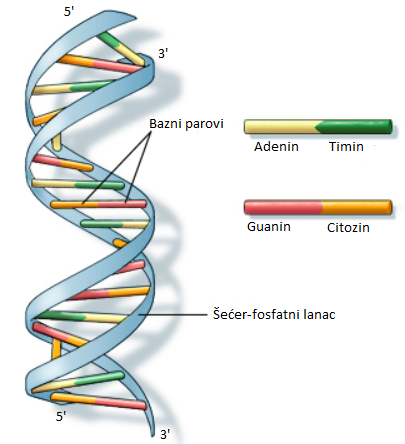
\includegraphics[width=0.7\textwidth]{dnk.PNG}
  \caption{Struktura DNK}
  \label{fig:00}
  \source{Izvor: \cite{DNA}}
\end{figure}

Molekul DNK se može zamisliti odmotan i rotiran, tako da su trake merdevina orijentisane vertikalno, a bazni parovi se mogu čitati sa leva na desno (slika \ref{fig:odmotanDnk}):

\begin{figure}[!ht]
  \centering
  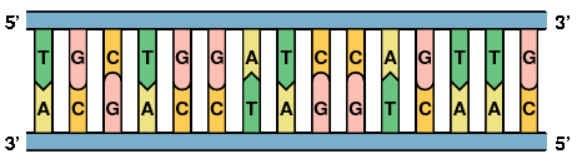
\includegraphics[width=0.7\textwidth]{odmotanDnk.PNG}
  \caption{Struktura DNK}
  \label{fig:odmotanDnk}
  \source{Izvor: \cite{DNA2}}
\end{figure}

U stvari, krajevi šećer-fosfatnih lanaca se međusobno razlikuju po prirodi nevezanog atoma ugljenika - jedan kraj ima nevezani $5'$ atom ugljenika, dok drugi kraj ima nevezani $3'$ atom ugljenika. Kada predstavljamo molekul DNK pomoću dijagrama, kakav je prikazan na slici \ref{fig:00}, podrazumeva se da gornji lanac kreće od $5'$ kraja sa leve strane do $3'$ kraja sa desne strane. Donji lanac je obrnuto orijentisan, od $3'$ kraja sa leve strane do $5'$ kraja sa desne strane \cite{DNA2}. 

\textbf{Geni} su delovi DNK sekvence koja je sa računarske strane niska nad azbukom $\{A, C, G, T\}$.  Svaki gen predstavlja pravilo za sintezu jednog proteina u ćeliji, koji je neophodan za njeno pravilno funkcionisanje. \textbf{Genom} je skup gena jednog organizma i sastoji od niza uparenih baza.

\textbf{Sekvenciranje genoma} podrazumeva otkrivanje sastava genoma. U pitanju je eksperimentalan
proces – da bi se saznalo šta se nalazi u sastavu jednog genoma, potreban je uzorak tkiva
odgovarajuće vrste \cite{skriptaBio}. \textbf{Sekvencioniranje DNK} je proces određivanja preciznog redosleda nukleotida unutar molekula DNK, a mašine koje određuju redosled nukleotida nazivaju se \textbf{sekvenceri}. Sekvencioniranje DNK uključuje bilo koji metod ili tehnologiju koja se koristi za određivanje redosleda četiri baze iz našeg genoma (A, C, G, T) \cite{DataAlgorithms}. Savremene laboratorijske metode za dati uzorak krvi pacijenta mogu da očitaju podsekvence DNK koje se nazivaju \textbf{očitavanja (engl. \textit{reads})}, a koje je nakon toga neophodno sastaviti u polaznu DNK sekvencu pomoću posebnih alata za sklapanje, takozvanih \textbf{asemblera}. Genomi i očitavanja DNK se mere u \textbf{baznim parovima (bp)}. Očitavanja mogu biti  \textbf{kratka} i \textbf{duga}. Kratka očitavanja imaju dužinu od 50 bp do 400 bp, a duga očitavanja dužinu veću od 400 bp.

Rekonstrukcija genoma kroz sekvencioniranje DNK je veoma važan problem. Ona se može uporediti sa kompletiranjem slagalice, gde su očitavanja delovi slagalice. Što su delovi veći, slagalicu je lakše sastaviti.

\begin{comment}
Rekonstrukcija genoma kroz sekvencioniranje DNK je veoma važan problem u genomici. Postojeće biotehnologije ne mogu proći kroz ceo hromozom, jer je predugačak. Umesto toga, genom se rekonstruiše indirektno. Prvo, vrši se razbijanje genoma na DNK fragmente koristeći pristup očitavanja celog sekvencioniranog genoma (engl. \textit{whole genome shotgun approach}). Zatim se pomoću mašine za sekvencioniranje na osnovu fragmenata vrši dekodiranje DNK sekvence. Ove DNK sekvence se nazivaju \textbf{očitavanja (engl. \textit{reads})}. Usled slučajnog uzorkovanja , ekstahovana očitavanja pokrivaju ceo genom ravnomerno. Lepljenjem ovih očitavanja možemo računski rekonstruisati genom. Ovaj proces je poznat kao \textbf{\textit{de novo} genomsko sekvencioniranje}.
\end{comment}

\newpage

\section{Istorija sekvencioniranja genoma}

\textbf{Sanger sekvencioniranje} predstavlja prvu tehniku sekvencioniranja. Nastala je 1977. godine, a njeni tvorci su Frederik Sanger (engl. \textit{Frederick Sanger}) i njegove kolege. Razvijena su dva asemblera za asembliranje očitavanja Sanger sekvencioniranja: \textit{OLC} \footnote{OLC je skraćenica od \textit{overlap layout consensus}, gde \textit{overlap} predstavlja izgradnju grafa preklapanja,
\textit{layout} spajanje putanja u grafu u kontige, a \textit{concensus} određivanje najverovatnije sekvence
nukleotida za svaku kontigu} asembler \textbf{Celera} i asembler \textbf{Ojler} zasnovan na De Brujinovim grafovima. \textbf{Humani referentni genom} sastavljen je korišćenjem ova dva pristupa. Humani referentni genom (poznat i kao referentni sklop) je digitalna baza podataka o nukleinskim kiselinama, koju su naučnici prikupili kao reprezentativni primer skupa gena čoveka. Kako su često sastavljeni sekvencioniranjem DNK većeg broja davalaca, referentni genomi ne predstavljaju skup gena nijedne pojedinačne osobe. Humani referentni genom \textit{\textbf{GRCh37}} \footnote{\textbf{GRCh37} - The Genome Reference Consortium human genome (build 37)} je izveden 2009. godine iz DNK trinaest anonimnih dobrovoljaca iz Bafala (engl. \textit{Buffalo}) (Njujork). Referentni genomi se obično koriste kao uputstvo na osnovu koga se grade novi genomi, što im omogućava da se sastave mnogo brže i ekonomičnije. Međutim, kako je Sanger sekvencioniranje niskopropusno (ima manju stopu greške) i ne tako ekonomično, samo nekoliko genoma je sastavljeno Sanger sekvencioniranjem.

Razvoj tehnika za sekvencioniranje \textbf{druge generacije} značajno je doprineo efikasnijem i sekvencioniraranju stotine miliona očitavanja. Međutim, očitavanja druge generacije sekvencioniranja su kratka. Po narudžbini su pravljeni genomski asembleri za rekonstrukciju genoma na osnovu kratkih očitavanja. Njihova pojava je dovela do većeg broja uspešnih \textbf{\textit{de novo}} asemblerskih projekata, uključujući rekonstrukciju genoma \textbf{Džejmsa Votsona} (engl. \textit{James Watson}) i \textbf{panda} genoma. Iako je ovaj pristup ekonomičan, rezultat su bili fragmentisani genomi, jer su očitavanja kratka i ponavljajući regioni, takozvani \textbf{ponovci} \footnote{Ponovci su fenomen kada se šablon od nekoliko nukleotida pojavljuje više puta u nizu.}, dugi.

Od nedavno su na raspolaganju tehnike za sekvencioniranje \textbf{treće generacije}, koje proizvode duga očitavanja (dužine od oko 10000 bp). Duga očitavanja mogu obuhvatiti složene genomske karakteristike, omogućavajući ispravnije postavljanje ovih karakteristika u rekonstruisanom genomu, tj. mogu rešiti problem ponavljajućih regiona. Međutim, duga očitavanja imaju visoku stopu greške $(15\%-18\%)$. U cilju rešavanja ovog problema razvijen je veliki broj računskih metoda za korekciju grešaka u očitavanjima treće generacije sekvencioniranja.

\newpage

\section{\textit{Shotgun} sekvencioniranje celokupnog genoma}

Prvi korak u procesu sekvencioniranja genoma je njegovo razbijanje na skup očitavanja, a na osnovu uzorka genoma. Postoji više vrsta očitavanja:
\begin{itemize}
    \item {jednostrana očitavanja (\textit{single-end reads})}
    \item {uparena očitavanja (\textit{paired-end reads})}
\end{itemize}

Posebna vrsta uparenih očitavanja su \textbf{partner-uparena očitavanja} (engl. \textit{mate-pair reads}). Prikaz svih vrsta očitavanja može se videti na slici \ref{fig:01}:

\begin{figure}[!ht]
  \centering
  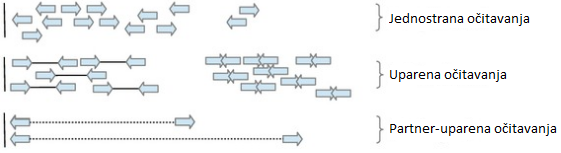
\includegraphics[width=\textwidth]{vrste_ocitavanja.PNG}
  \caption{Vrste očitavanja}
  \label{fig:01}
  \source{Izvor: \cite{WingKinSung}}
\end{figure}

Sekvenceri čitaju deo DNK fragmenta neke unapred
zadate dužine koja se naziva \textbf{dužina očitavanja}. \textbf{Dubina pokrivanja} neke pozicije u DNK sekvenci je velika, ako je nukleotid na toj poziciji pročitan veliki broj puta u jedinstvenim očitavanjima. Tačnost sekvencioniranja za svaki pojedinačni nukleotid je veoma visoka, ali ukoliko se pojedinačni genom sekvencira samo jednom, zbog veoma velikog broj nukleotida u genomu doći ć́e do značajnog broja grešaka u sekvencioniranju. Pored toga, mnoge pozicije u genomu sadrže retke \textbf{jednonukleotidne polimorfizme} \footnote{Pojava zamene mesta jednog nukleotida nekim drugim nukleotidom} (engl. \textit{single-nucleotide polymorphisms - SNPs}). Stoga, kako bi se napravila razlika između grešaka u sekvencioniranju i pravih SNP-ova, potrebno je još više poveć́ati tačnost sekvencioniranjem pojedinačnih genoma veći broj puta \cite{SequencingCoverage}.

Za potrebe \textit{shotgun} sekvencioniranja celokupnog genoma postoje dva protokola: 
\begin{itemize}
    \item {sekvencioniranje celokupnog genoma}
    \item {sekvencioniranje partner-uparenih očitavanja}
\end{itemize}

\newpage

\subsection{Sekvencioniranje celokupnog genoma}

Sekvencioniranje celokupnog genoma uključuje tri koraka koja su prikazana na slici \ref{fig:1}:

% Uključuje 3 koraka: (1) korak razbijanja genoma (\textit{sonication}), (2)
% korak odabira dužine očitavanja i izdvajanja fragmenata te dužine (\textit{size selection}), (3) korak očitavanja kraj(ev)a svakog fragmenta (\textit{sequencing})

\begin{figure}[!ht]
  \centering
  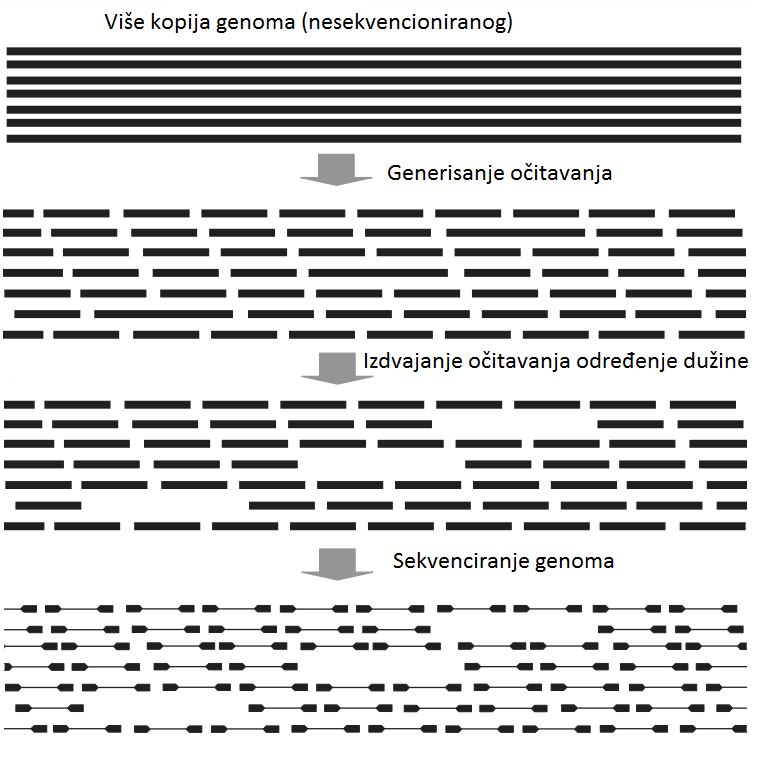
\includegraphics[width=0.8\textwidth]{prva.png}
  \caption{Ilustracija protokola \textit{shotgun} za sekvencioniranje celokupnog genoma.}
\label{fig:1}
\source{Izvor: \cite{WingKinSung} str. 122, slika 5.1}
\end{figure}

Prvo, uzorak genoma se na slučajan način razbija na DNK fragmente. Zatim sledi korak odabira dužine očitavanja u kom se vrši ekstrahovanje DNK fragmenata te dužine. Na kraju se vrši sekvencioniranje jednostranih očitavanja ili sekvencioniranje uparenih očitavanja. Pri sekvencioniranju jednostranih očitavanja, sekvencer čita DNK fragment u jednom smeru, dok u slučaju uparenih očitavanja, fragment biva pročitan u oba smera.

Na slici \ref{fig:2} prikazan je odmotan i rotiran DNK fragment ekstrahovan iz uzorka genoma:

\begin{figure}[!ht]
  \centering
  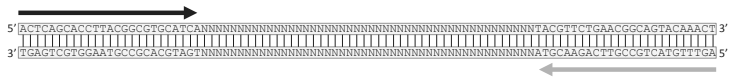
\includegraphics[width=\textwidth, height=2.4cm]{druga.PNG}
  \caption{DNK fragment ekstrahovan iz uzorka genoma}
  \label{fig:2}
  \source{Izvor: \cite{WingKinSung} str. 122, slika 5.2}
\end{figure}

 Za sekvencioniranje jednostranih očitavanja, dobija se očitavanje sa 5' kraja \footnote{$5'$ i $3'$ označavaju brojeve ugljenika koji se nalaze u osnovi DNK šećera. $5'$ ugljenik ima fosfatnu grupu koja je vezana za njega, a $3'$ ugljenik-hidroksilnu (-OH) grupu. Ova asimetrija daje DNK pravac $5' \rightarrow 3'$. Na primer, DNK polimeraza deluje u pravcu $5' \rightarrow 3'$, tj. dodaje nukleotide na $3'$ kraj molekula napredujući u tom smeru.} gornjeg lanca, tj. $ACTCAGCACCTTACGGCGTGCATCA$. Za sekvencioniranje uparenih očitavanja, dobijaju se $5'$ očitavanja i gornjeg i donjeg lanca, pri čemu je drugo očitavanje inverzni komplement prvog, tj:

\begin{itemize}
    \item {$ACTCAGCACCTTACGGCGTGCATCA$}
    \item {$AGTTTGTACTGCCGTTCAGAACGTA$}
\end{itemize}

Za asembliranje genoma, dužina očitavanja je veoma važan parametar. Različite tehnologije sekvencioniranja imaju različita ograničenja na dužinu očitavanja. Na primer, \textit{Illumina Hi-seq} \footnote{Illumina je američka kompanija koja je proizvodila sekvencere sa malom stopom greške (engl. \textit{high-throughput sequencers})} sekvencioniranje može izvršiti samo sekvencioniranje uparenih očitavanja dužine manje od 1000 bp. Za treću generaciju sekvencioniranja, ograničenje dužine očitavanja može biti veće od 10000 bp.

\newpage

\subsection{Sekvencioniranje partner-uparenih očitavanja}

Sekvenceri druge generacije mogu izdvojiti partner-uparena očitavanja sa oba kraja kratkih fragmenata DNK (dužine očitavanja manje od 1000 bp). Za izdvajanje ovakvih očitavanja možemo koristiti \textbf{sekvencioniranje partner-uparenih očitavanja} prikazano na slici \ref{fig:3} :

%Slika 2.3 i opis Figure 5.3 iz knjige
\begin{figure}[!ht]
  \centering
  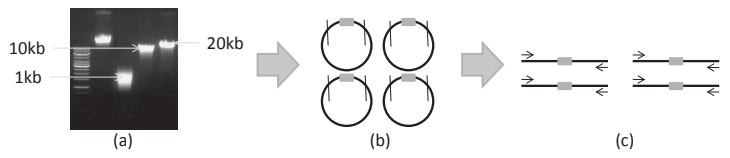
\includegraphics[width=0.8\textwidth, height=3cm]{treca.PNG}
  \caption{Ilustracija protokola sekvencioniranja partner-uparenih očitavanja}
\source{Izvor: \cite{WingKinSung} str. 123, slika 5.3}
\label{fig:3}
\end{figure}

 Prvo se izdvajaju dugi DNK fragmenti neke fiksirane dužine očitavanja (npr. 10000 bp) (slika \ref{fig:3}(a)). Svaki DNK fragment se cirkularizuje pomoću adaptera \footnote{Adapter sekvence su kratke hemijski sintetizovane sekvence
nukleotida koje se mogu vezati za krajeve nepoznatih DNK sekvenci i neophodne su u nekim koracima sekvencioniranja.} (blok sive boje) (slika \ref{fig:3}(b)). Zatim se vrši sečenje fragmenta levo i desno od adaptera. Na kraju se uparena očitavanja ekstrahuju sekvencioniranjem uparenih očitavanja (slika \ref{fig:3}(c)).

Orijentacije uparenih očitavanja očitanih od strane sekvencera partner-uparenog i uparenog očitavanja se razlikuju. Sekvenceri partner-uparenih očitavanja daju dva očitavanja sa oba kraja svakog fragmenta DNK u spoljašnjoj orijentaciji umesto u unutrašnjoj. Npr. za DNK fragment na slici \ref{fig:2} sekvencioniranje partner-uparenih očitavanja će dati:
\begin{itemize}
    \item {TGATGCACGCCGTAAGGTGCTGAGT}
    \item {TACGTTCTGAACGGCAGTACAAACT}
\end{itemize}

Iako protokol za sekvencioniranje partner-uparenih očitavanja može izdvojiti uparena očitavanja velike dužine očitavanja, on zahteva veći broj ulaznih kopija genoma za pripremu sekvencerskih biblioteka i sklon je lažnim greškama.

\section{\textit{De novo} sekvencioniranje genoma za kratka očitavanja}

Druga generacija tehnika sekvencioniranja omogućava dobijanje skupa jednostranih ili uparenih kratkih očitavanja celokupnog genoma. \textit{De novo} sekvencioniranje ima za cilj da izvrši preklapanje očitavanja u ispravnom redosledu i rekonstruiše genom.

Problem asembliranja genoma je računski težak. Čak i kada ne postoji greška sekvencioniranja, ovaj problem je ekvivalentan \textbf{problemu suprstringa} za koji se zna da je NP-kompletan (problem superstringa - na osnovu skupa stringova $S$, teži se pronalaženju superstringa, najkraćeg stringa $P$ takavog da je svaki string $s$ iz skupa $S$ substring stringa $P$. Na primer, ako je $S = \{ACATGC, ATGCGTGT, GTGTACGT\}$, onda je superstring ACATGCGTGTACGT).

Mnogi \textit{de novo} asembleri \footnote{De novo asembleri su programi
koji vrše sklapanje tako što proširuju kratka očitavanja spajanjem susednih
očitavanja u dužu sekvencu, bez korišćenja referentne sekvence} predlažu asembliranje kratkih očitavanja. Opšte rešenje uključuje 4 koraka prikazana na slici \ref{fig:4}:

% Figure 5.4 i slika 2.4
\begin{figure}[!ht]
  \centering
  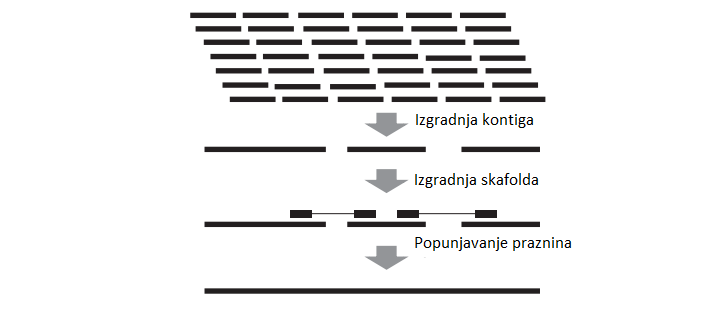
\includegraphics[width=\textwidth,height=8cm]{cetvrta.PNG}
  \caption{Četiri koraka u \textit{de novo} sekvencioniranju genoma}
  \label{fig:4}
  \source{Izvor: \cite{WingKinSung} str. 124, slika 5.4}
\end{figure}

U prvom koraku se koriguju greške sekvencioniranja u očitavanjima. Na osnovu korigovanih očitavanja, u drugom koraku se vrši spajanje očitavanja preklapanjem. U idealnom slučaju, teži se spajanju svih očitavanja tako da se formira kompletan genom, ali kako se zbog ponovaka javljaju dvosmislenosti, to nije moguće. Postojeće metode preklapanjem očitavanja grade kontinuiranu sekvencu, takozvanu \textbf{kontigu} (engl. \textit{contig}). Kontige obično predstavljaju jednu \textbf{konsenzus nisku} \footnote{Niska sastavljena od najfrekventnijih nukleotida na pozicijama poravnatih sekvenci}. Zatim, koristeći uparena očitavanja, pokušava se rekonstrukcija redosleda kontiga tako da se formiraju \textbf{skafoldi} (engl. \textit{scaffolds}). Svaki skafold je niz kontiga, a jos se naziva i \textbf{superkontig} ili \textbf{metakontig}. Na kraju se vrši preuređivanje očitavanja u skafoldima kako bi se popunile praznine između susednih kontiga.

\section{Korekcija grešaka}

Greške u sekvencioniranju očitavanja dovode do novih k-mera koji se pojavljuju mnogo ređe od ispravnih k-mera, dok se k-meri izvučeni iz sekvenci koje se ponavljaju u genomu (poput prenosnih elemenata) pojavljuju mnogo češće nego k-meri sa jednom kopijom (preformulisati). Ove razlike se mogu iskoristiti za filtriranje grešaka u k-merima i selektivno uklanjanje očitavanja koja sadrže greške sekvencioniranja iz skupa podataka. (citiranje)
Greške u sekvencioniranju očitavanja mogu zbuniti \textit{de novo} asemblere. Da bi se to izbeglo, vrši se korigovanje tih grešaka pre početka asembliranja genoma.

\subsection{Brojanje k-mera}

Jedan konceptualno jednostavan, ali osnovni problem je \textbf{brojanje k-mera} \footnote{Podniska dužine k}. To je potprogram koji se koristi u korekciji grešaka u očitavanjima. Može biti korišćen i u koraku asembliranja, detekciji ponovaka i kompresiji genomskih podataka. Ima značajnu ulogu u utvrđivanju da li je došlo do grešaka u sekvencioniranju ili je u pitanju jednonukleotidni polimorfizam. Ulaz u ovaj potprogram je skup očitavanja $R$ i parametar $k$. Neka je $Z$ skup svih mogućih k-mera koji se pojavljuju u $R$. Problem je izračunavanje frekvencije pojavljivanja k-mera u $Z$. U nastavku će biti razmatrana 4 rešenja: \textbf{(1) jednostavno heširanje, (2) JellyFish, (3) BFCounter i (4) DSK.}

\newpage

\subsubsection{Jednostavno heširanje}
Problem brojanja k-mera može biti rešen implementacijom asocijativnog niza koristeći \textbf{heširanje} \footnote{Tehnika kojom se vrsi preslikavanje skupa ključeva na tabelu značajno manjih dimenzija. Idealno bi bilo da funkcija za svaki ključ
daje jedinstvenu poziciju. Ta funkcija naziva se heš funkcija, a tabela koja se koristi u tom
postupku zove se heš tabela.}. Kada je $k$ malo (npr. manje od 10), koristi se \textbf{savršeno heširanje}. Savršeno heširanje garantuje da neće doći do \textbf{kolizije}  \footnote{Izraz koji potiče od latinske reči \textit{collisio} i znači sudar, sukob. U ovom kontekstu, moguće je da heš funkcija za dva razlicita k-mera da istu vrednost, te kažemo da su ta 2 k-mera u koliziji, tj. sukobu.}. To je moguće kada se tačno zna koji skup ključeva će biti heširan prilikom dizajniranja heš funkcije. Svaki k-mer $z$ može biti kodiran kao 2k-bitni binarni ceo broj \textit{b(z)} zamenom $A$, $C$, $G$ i $T$ u $z$ sa 00, 01, 10, 11, respektivno. Tako se izgrađuje tabela $Count[0..4^k - 1]$ veličine $4^k$ u kojoj svaka ulazna vrednost $Count[b(z)]$ čuva frekvenciju k-mera $z$ u skupu $Z$. Preciznije, vrši se inicijalizacija svake ulazne vrednosti u $Count[0..4^k - 1]$ na 0. Zatim se iterativno skenira svaki k-mer $z$ iz $Z$ i uvećava $Count[b(z)]$ za 1. Na kraju, sve ulazne vrednosti različite od nule u $Count[]$ predstavljaju k-mere koji se pojavljuju u $Z$ kao i broj njihovih pojavljivanja.
\begin{comment}
Slika \ref{fig:5}(a) predstavlja primer koji ilustruje ovaj jednostavni metod prebrojavanja:

\begin{figure}[!ht]
  \centering
  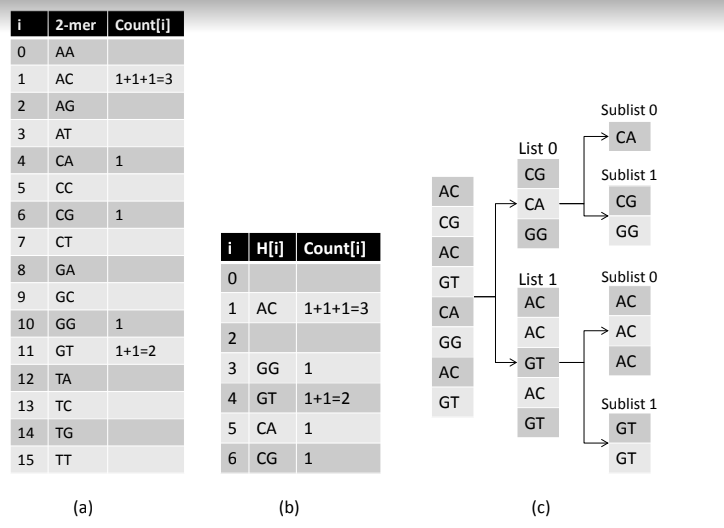
\includegraphics[width=\textwidth]{58_3algoritma.PNG}
  \caption{Razmatra se skup 4-mera $Z = \{AC; CG; AC; GT; CA; GG; AC; GT\}$: (a) Ilustruje jednostavan metod za brojanje k-mera koji koristi \textit{Count} tabelu veličine 4k. (b) Ilustruje \textit{JellyFish} metod brojanja k-mera koja koristi heš tabelu veličine 7. Heš funkcija je $h(z) = b(z)$ \textit{mod} $7$. Na primer, $GT$ se čuva u tabeli $Count$ sa indeksom 4, jer je $h(GT) = 4$. U ovom primeru se javlja je DNK kolizija. Pošto je i $h(CA) = 4$, $CA$ je u koliziji sa $GT$. Linearnim isprobavanjem $CA$ se ipak čuva u tabeli $Count$ sa indeksom 5. (c) Ilustruje DSK metod brojanja k-mera.
Pretpostavka je da je $h(z) = b(z)$, $n_{list} = 2$ i $n_{sublist} = 2$. DSK deli Z u
4 ($= n_{list} * n_{sublist}$) podliste, a zatim pokreće \textit{JellyFish} algoritam za brojanje k-mera u svakoj podlisti.}
  \label{fig:5}
  \source{\cite{WingKinSung} str. 131, slika 5.8}
\end{figure}

\end{comment}

Neka je $N = |Z|$. Tada je navedeni pristup veoma efikasan. Njegovo vreme izvršavanja je $O(N + 4^k)$, a kako treba izgraditi tabelu veličine $4^k$, prostorna složenost je $O(4^k)$. Kada je $k$ veliko, navedeni algoritam ne može da radi, jer zahteva previše prostora.


\subsubsection{JellyFish algoritam}
Moguće je smanjiti veličinu heš tabele koristeći mehanizam \textbf{otvorenog adresiranja}. Otvoreno adresiranje je način rešavanja kolizije u heš tabelama. Kada se desi kolizija, traži se sledeća slobodna lokacija u heš tabeli za smeštanje vrednosti. Postoje 3 metode otvorenog adresiranja: \textbf{linearno popunjavanje}, \textbf{kvadratno popunjavanje} i \textbf{duplo heširanje}. Neka je $h()$ heš funkcija i $H[0..\frac{N}{\alpha} - 1]$ heš tabela koja čuva niz k-mera, gde je $\alpha$ \textbf{faktor opterećenja}  \footnote{Broj koji kontroliše veličinu heš tabele} $(0 < \alpha \leq 1)$. Potrebno je izgraditi tabelu $Count[0..\frac{N}{\alpha} - 1]$ gde $Count[i]$ čuva broj pojavljivanja za k-mer $H[i]$. Za svaki k-mer iz $Z$ vrši se njegovo  heširanje u neku vrednost $H[i]$ gde je $i = h(z)$. Ako $H[i]$ nije prazan i $H[i] \neq z$, ne možemo čuvati $z$ u $H[i]$, tj. došlo je do kolizije. Ona može biti razrešena pomoću mehanizma otvorenog adresiranja. Na primer, kolizija se može razrešiti \textbf{linearnim popunjavanjem}. Ovom metodom pokušavamo da uvećamo indeks $i$ za jedan kada se kolizija dogodi sve dok je $H[i] = z$ ili je ulaz $H[i]$ prazan. Nakon sto su svi k-meri iz $Z$ obrađeni i sve kolizije razrešene, prikazuje se $(H[i], Count[i])$ za sve ulaze $H[i]$ različite od nule.
\begin{comment}
Funkcija $hashEntry()$ sa slike \ref{fig:6} (donji deo slike) ilustruje šemu linearnog popunjavanja za razrešavanje kolizije. Ako $hashEntry(z, h, \frac{N}{\alpha})$ vraća prazan ulaz $H[i]$, onda $z$ ne postoji u heš tabeli i postavljamo $H[i] = z$ i $Count[i] = 1$. U suprotnom, ako $hashEntry(z, h, \frac{N}{\alpha})$ vraća ulaz $H[i] = z$, uvećavamo $Count[i]$ za jedan. Nakon sto su svi k-meri iz $Z$ obrađeni, prikazujemo $(H[i], Count[i])$ za sve ulaze $H[i]$ različite od nule.

JellyFish algoritam je detaljnije objašnjen na slici \ref{fig:6} (gorni deo slike), dok slika \ref{fig:5} (b) daje primer koji ga ilustruje. On je efikasniji, ukoliko ne postoji kolizija. U praksi je očekivani broj kolizija manji, ukoliko za faktor opterećenja važi $\alpha \leq 0.7$. Zatim, očekivano vreme izvršavanja je $O(N)$. Što se tiče prostorne složenosti, tabele $H[]$ i $Count[]$ zahtevaju $\frac{N}{\alpha}(2k + 32)$ bitova, pod pretpostavkom da broj zauzima 32 bita. Gore pomenuta ideja smanjivanja veličine heš tabele je iskorišćena u $JellyFish$ algoritmu.

\begin{figure}[!ht]
  \centering
  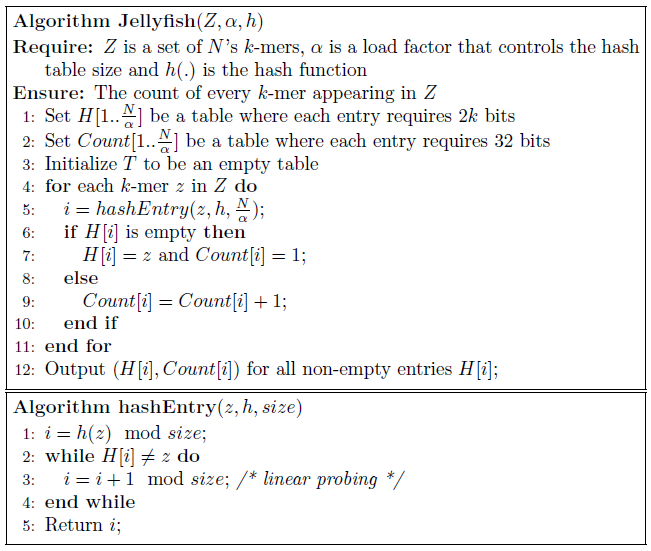
\includegraphics[width=0.85\textwidth]{Jellyfish5_9.PNG}
  \caption{Jellyfish algoritam i funkcija hashEntry}
  \label{fig:6}
  \source{\cite{WingKinSung} str. 132, slika 5.9}
\end{figure}

\end{comment}

Iako $JellyFish$ algoritam koristi manje prostora od metode naivnog prebrojavanja, $JellyFish$ heš tabela mora biti veličine koja je jednaka bar broju jedinstvenih k-mera iz $Z$. $JellyFish$ i dalje zahteva mnogo memorije u slučaju da je broj jedinstvenih k-mera u $Z$ veliki.

\subsection{BFCounter algoritam}
U mnogim aplikacijama, od značaja su samo k-meri koji se pojavljuju najmanje $q$ puta. Kada bi moglo da se izbegne čuvanje k-mera koji se pojavljuju manje od $q$ puta, sačuvalo bi se mnogo memorije. Pol Melsted (engl. \textit{Páll Melsted}) je predložio algoritam  \textbf{BFCounter} koji broji samo k-mere koji se pojavljuju najmanje $q$ puta. On koristi \textit{counting Bloom} filter da odredi da li se k-mer pojavljuje najmanje $q$ puta. To je prostorno efikasna probabilistička struktura podataka koja dozvoljava dodavanje bilo kojih k-mera u nju i ispitivanje da li se k-mer pojavljuje najmanje $q$ puta. Iako on može dati pogrešno pozitivan rezultat (pogrešan izveštaj da k-mer postoji ili pogrešno proceniti broj k-mera), ne može dati pogrešno negativan rezultat. \textit{BFCounter} održava \textit{counting Bloom} filter $B$ i heš tabelu $H$ i sastoji od 2 faze. 

Prva faza počinje sa praznim \textit{counting Bloom} filterom $B$ i praznom heš tabelom $H$. U ovoj fazi se skeniraju k-meri iz $Z$ jedan po jedan. Za svaki k-mer $z\inZ$ se proverava da li se $z$ pojavljuje najmanje $q - 1$ puta u \textit{counting Bloom} filteru $B$ utvrđivanjem da li je $countBloom(x, B) \geq q-1$. Ako nije, vrši se umetanje $z$ u $Z$ pomoću $insertBloom(z, B)$. U suprotnom, $z$ se pojavljuje najmanje $q$ puta. Zatim se vrši proveravanje da li je $z$ u heš tabeli $H$. Ako nije, $z$ se umeće u neki prazan ulaz $H[i]$ i postavlja se $Count[i]$ na nulu. 

U drugoj fazi se obavlja stvarno brojanje. Vrši se skeniranje k-mera iz $Z$ jedan po jedan. Za svaki k-mer $z$ iz $Z$, ako se $z$ pojavljuje u heširanom ulazu $H[i]$, onda se uvećava $Count[i]$ za 1.

\begin{comment}

Detaljan pseudokod je prikazan na slici \ref{fig:7}:

%Figura 5.10
\begin{figure}[h]
\centering
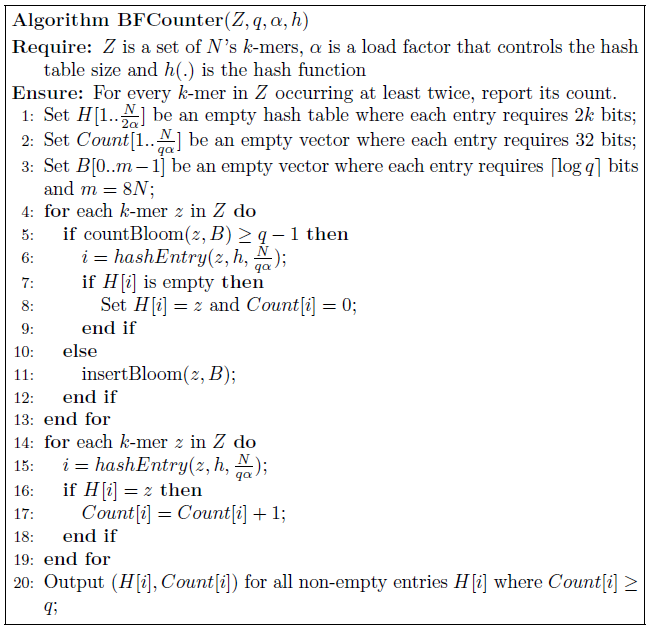
\includegraphics[width=12cm]{BFCounter5_10.PNG}
\caption{Prostorno efikasan algoritam za prebrojavanje k-mera koji broji samo k-mere koji se pojavljuju najmanje q puta.}
\label{fig:7}
\source{\cite{WingKinSung} str. 134, slika 5.10}
\end{figure}

\end{comment}

Vreme izvršavanja \textit{BFCounter} algoritma je $O(n)$. Što se tiče prostorne složenosti, \textit{counting Bloom} filter zahteva $O(N log(q))$. Prostor za $H[]$ i $Count[]$ je $\frac{N'}{\alpha}(2k + 32)$ bitova, gde je $N'$ broj k-mera koji se pojavljuju najmanje $q$ puta. Primetimo da je $N' \leq \frac{N}{q}$.

\newpage

\subsection{DSK algoritam}
Iako je BFCounter prostorno efikasan, njegova prostorna složenost i dalje zavisi od broja $N$ k-mera u $Z$. Neka je memorija fiksirana tako da bude $M$ bitova i neka je memorija diska fiksirana tako da bude $D$ bitova. Da li se može i dalje efikasno izračunati pojavljivanja k-mera? Gijom Rizk (engl. \textit{Guillaume Rizk}) nam daje pozitivan odgovor i predlaže metod koji se naziva \textbf{DSK}

\begin{comment}

, a čiji pseudokod je prikazan na slici \ref{fig:63}:

%Figura 5.11
\begin{figure}[h]
\centering
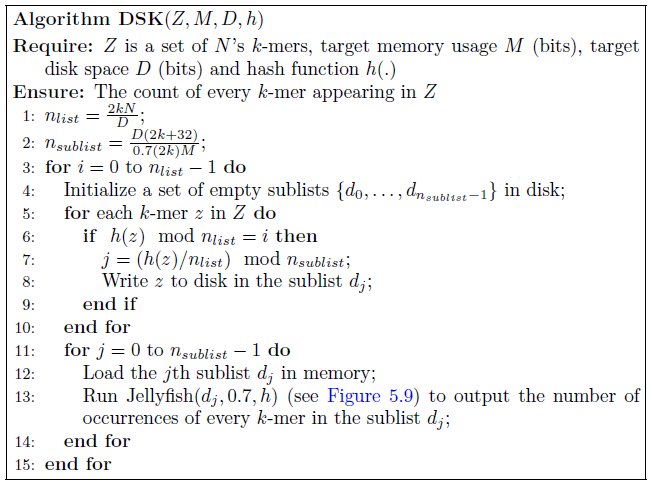
\includegraphics[width=12cm]{DSK5_11.PNG}
\caption{DSK algoritam}
\label{fig:63}
\source{\cite{WingKinSung} str. 136, slika 5.11}
\end{figure}

\end{comment}

Ideja ovog metoda je da se skup k-mera $Z$ podeli u različite liste tako da svaka lista bude smestena na disk koristeći $D$ bitova. Zatim, za svaku listu, k-meri iz liste se dalje dele u podliste tako da svaka podlista može biti sačuvana u memoriji koristeći $M$ bitova. Na kraju, frekvencije k-mera u svakoj podlisti se izračunavaju algoritmom $JellyFish$.

\begin{comment}
Preciznije, k-meri u $Z$ su podeljeni u $n_{list}$ lista približno slične dužine. Kako disk ima $D$ bitova i svaki k-mer može biti reprezentovan u 2k bitova, svaka lista može čuvati $l_{list} =  \frac{D}{2k}$ k-mera. Kako imamo $N$ k-mera u $Z$, postavlja se $n_{list} = \frac{N}{n_{list}} = \frac{2kN}{D}$. Ovo deljenje se obavlja heš funkcijom $h()$ koja ravnomerno mapira sve k-mere u $n_{list}$ lista. Preciznije, za svaki k-mer $z$ iz $Z$, $z$ se dodeljuje i-toj listi, ako je $h(z)$ \textit{mod} $n_{list} = i$. 

Zatim, svaka lista se dalje deli u podliste, pri čemu je svaka dužine $l_sublist$. Svaka podlista će biti obrađena u memoriji pomoću algoritma $JellyFish$, koji zahteva $\frac{l_{sublist}}{0.7}(2k +32)$ bitova. Kako memorija ima $M$ bitova, tako je $l_{sublist} = \frac{0.7M}{(2k + 32)}$.

Broj podlista je jednak $n_{sublist} = \frac{n_{list}}{n_{sublist}} = \frac{D(2k + 32)}{0.7(2k)M}$. Slično, svaka lista je podeljena u podliste heš funkcijom $h()$. Preciznije, za svaki k-mer $s$ u i-toj listi, $s$ je dodeljeno j-toj podlisti, ako je $(\frac{h(s)}{n_{list}})$ \textit{mod}
$n_{sublist} = j$.

Za svaku podlistu dužine $l_{sublist} = {0.7M}{2k + 32}$, koristeći $M$ bitova,  brojimo pojavljivanja svakog k-mera u podlisti koristeći $JellyFish(d_j, 0.7, h)$ sa slike \ref{fig:6}.

Na slici \ref{fig:5}(c) se može videti primer koji ilustruje izvršavanje algoritma DSK. Neka je $n_{list} = 2$, $n_{sublist} = 2$ and $h(z) = b(z)$ za svaki $z \in Z$. Kako je $n_{list} = 2$, algoritam izvršava 2 iteracije (u nastavku sledi opis nulte iteracije, jer se prva izvršava slično). Prva faza nulte iteracije skenira sve k-mere iz $Z$ i identifikuje svaki k-mer $z \in Z$ koji pripada nultoj listi. Na primer, $h(GG) = 10$, kako je $h(GG)$ \textit{mod} $n_{list} = 0$ i $\frac{h(z)}{n_{list}}$ \textit{mod} $n_{sublist} = 1$, $GG$ pripada nultoj listi i prvoj podlisti. Nakon toga, nulta lista se deli na nultu podlistu $\{CA\}$ i prvu podlistu $\{CG, GG\}$. Obe podliste su zapisane na disku. Druga faza čita svaku podlistu iz memorije i broji k-mere koristeći $JellyFish$ algoritam.

\end{comment}

Ovaj algoritam će zapisati samo jednom svaki k-mer iz $Z$, iako će svaki k-mer pročitati $n_{list}$ puta. Stoga, on neće generisati mnogo pristupa disku radi pisanja. Što se tiče vremenske složenosti, za i-tu iteraciju, algoritam numeriše sve k-mere u $Z$, što oduzima $O(n)$ vremena. Zatim, algoritam identifikuje $\frac{D}{2k}'s$ k-mera koji pripadaju i-toj listi i zapisuje ih na disk, što oduzima $O(\frac{D}{k})$ vremena. Nakon toga, algoritam  čita $\frac{D}{2k}'s$ k-mera i izvodi brojanje, što oduzima $O(\frac{D}{k})$ vremena. Tako da svaka iteracija zahteva $O(N + \frac{D}{k}) = O(N)$ vremena, gde je $N > \frac{D}{2k}$. Kako je $n_{list} = \frac{2kN}{D}$ broj iteracija, algoritam se izvršava u $O(kN^2)$ očekivanom vremenu. Kad je $D = \theta(N)$, algoritam se izvršava u $O(kN)$ očekivanom vremenu.

\newpage

\section{Konstrukcija kontiga}

Nakon što su sva očitavanja korigovana, može se vršiti njihovo spajanje radi formiranja kontiga. Postoje 2 pristupa za konstrukciju kontiga:
\begin{itemize}
    \item{pristup baznog proširenja (\textit{base-by-base} pristup)}
    \item{De Brujinov grafovski pristup}
\end{itemize}

\subsection{Pristup baznog proširenja}

Pristup baznog proširenja rekonstruiše svaku kontigu tako što je proširuje bazu po bazu. Metod počinje tako što se nasumično bira očitavanje koje će služiti kao šablon. Zatim se očitavanja poravnavaju na oba kraja šablona ($5'$ kraj i $3'$ kraj). Na osnovu poravnanja se dobija \textbf{konsenzusna baza} \footnote{Baza koja se pojavljuje najveći broj puta na određenoj poziciji u poravnanju.} i šablon se njome proširuje. Slika \ref{fig:7} ilustruje jedan korak baznog proširenja:

%Figure 5.12
\begin{figure}[!ht]
  \centering
  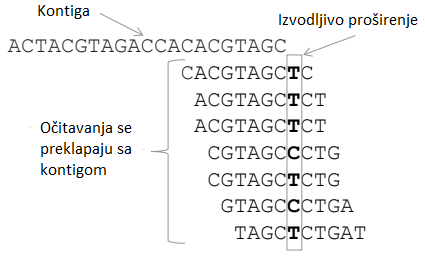
\includegraphics[width=0.8\textwidth]{contig5_12.PNG}
\caption{Jedan korak baznog proširenja}
\label{fig:7}
\source{\cite{WingKinSung} str. 137, slika 5.12}
\end{figure}

Gornja sekvenca predstavlja šablon, dok su ostalih sedam očitavanja poravnata na $3'$ kraju šablona. Pravougaonik pokazuje da su baze $C$ i $T$ izvodljivo proširenje šablona. Kako je $T$ konsenzusna baza, metod baznog proširenja će proširiti kontigu bazom $T$. Bazno proširenje se ponavlja sve dok ima konsenzusa. Zatim se prestaje sa proširenjem i dobija se kontiga. Proširenje se izvodi i na $3'$ kraju i na $5'$ kraju šablona.

\begin{comment}
Slika \ref{fig:8} daje pseudokod ovog metoda:

%Figure 5.13
\begin{figure}[!ht]
\centering
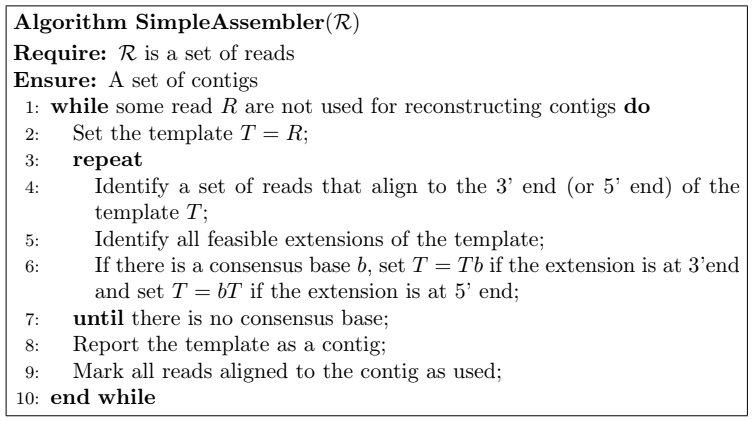
\includegraphics[width=0.9\textwidth]{SimpleAsembler5_13.PNG}
\caption{Jednostavan base-by-base asembler proširenja}
\label{fig:8}
\source{\cite{WingKinSung} str. 138, slika 5.13}
\end{figure}

\end{comment}

Iako je bazno proširenje jednostavno, ono često daje kratke kontige zbog dva problema. Prvo, početni šablon je nasumično izabrano očitavanje. Ukoliko ono sadrži greške sekvencioniranja ili se nalazi u ponovku, to će uticati na proširenje. Drugi problem je što se može desiti da se šablon proširi u neki od ponovaka. Ponovak stvara grane koje gore navedeni pristup ne može da razreši.

\begin{comment}
Da bismo rešili prvi problem, biramo očitavanje za šablon, ako je malo verovatno da ono sadrži grešku sekvenciranja ili ako je malo verovatno da će biti u ponovljenom regionu. Koristeći ideju u sekciji 5.3.1, broje se frekvencije svih k-mera svih očitavanja. Očitavanje R se bira za šablon, ako su frekvencije svih njegovih k-mera unutar nekih korisnički definisanih pragova $\theta_{min}$ i $\theta_{max}$. Ako je broj pojavljivanja nekog k-mera manji od $\theta_{min}$, R će verovatno sadržati grešku sekvenciranja. Ako je broj pojavljivanja nekog k-mera veći od $\theta_{max}$, R će se verovatno naći u ponovljenom regionu. Ova dva praga mogu biti određena proučavanjem histograma frekvencija svih k-mera ulaznih sekvenci očitavanja.

Za drugi problem, rešenje je korišćenje informacija o povezivanju paired-end očitavanja za rešavanje nasumičnosti. Ovaj pristup je korišćen od strane $PE-asemblera [9]$. Figura 5.14 ilustruje tu ideju. Pretpostavimo da možemo proširiti šablon koristeći 2 različita očitavanja (crno i sivo). Ne možemo odlučiti koje je ispravo (pogledati Figuru 5.14(a)). Kako svako očitavanje ima svog para, možemo biti u stanju da donesemo odluku. Postoje 2 slučaja. U prvom slučaju, ako parnjak crnom očitavanju može biti poravnat sa šablonom, možemo verovati crnom očitavanju (Figura 5.14(b)). U drugom slučaju, pretpostavimo  da postoji nekoliko očitavanja R koja su poravnata sa šablonom i parnjaci od R mogu biti poravnati sa panjakom crnog očitavanja (pogledati Figuru 5.14(c)). Onda možemo verovati i crnom očitavanju. Drugim rečima, informacije o povezanosti paired-end očitavanja mogu pomoći u  filtriranju onih lažno pozitivnih poravnanja.
\end{comment}

\subsection{De Brujinov grafovski pristup}

\textbf{De Brujinov grafovski pristup} je zasnovan na De Brujinovim grafovima. Ovaj pristup su uveli Induri (engl. \textit{Indury}) i Voterman (engl. \textit{Waterman}) u njihovoj knjizi \textit{"A new algorithm for DNK sequence assembly: Journal of Computational Biology"}. On je danas glavni pristup za asembliranje kratkih očitavanja.

Neka je dat skup očitavanja $R$ i parametar $k$. De Brujinov graf je graf $H_k = (V, E)$, gde je $V$ skup svih k-mera skupa $R$. Ako su $u$ i $v$ prefiks dužine $k$ i sufiks dužine $k$ neke podniske dužine $k + 1$ iz $R$, respektivno, k-meri $u$ i $v$ formiraju granu $(u, v) \in E$. Pod pretpostavkom da je $N$ ukupna dužina svih očitavanja iz $R$, De Brujinov graf može biti konstruisan u $O(N)$ vremenu.

Na primer, neka je dat skup stringova $R = \{ACGC, CATC, GCA\}$ i neka je potrebno izgraditi De Brujinov graf za date k-mere. Tada je skup čvorova $\{AC, AT, \\ CA, CG, GC, TC\}$. Slika \ref{fig:9}(a) daje prikaz De Brujinovog grafa:

%Figura 5.15
\begin{figure}[!ht]
\centering
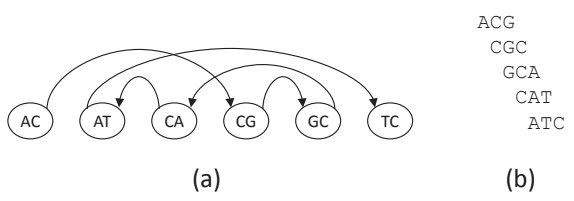
\includegraphics[width=0.7\textwidth]{Figura5_15.PNG}
\caption{(a) De Brujinov graf $H_3$ za $R = \{ACGC, CATC, GCA\}$. (b)
 Preklapanje 5 3-mera koji odgovaraju granama grafa $H_3$.}
 \label{fig:9}
 \source{\cite{WingKinSung} str. 139, slika 5.15}
 \end{figure}

Uzorak genoma se može predvideti identifikovanjem \textbf{Ojlerove putanje} \footnote{Ojlerova putanja je putanja koja obilazi svaku granu grafa $H_k$ tačno jednom.} grafa $H_k$. Ojlerova putanja grafa $H_k$ može biti izračunata u $O(n)$ vremenu, ako $H_k$ ima $n$ grana. Na primer, na slici \ref{fig:9}(a) postoji jedinstvena putanja od čvora $AC$ do čvora $TC$. Preklapanjem svih ivica 3-mera u redosledu putanje (slika \ref{fig:9}(b)) dobija se sekvenca $ACGCATC$. Sekvenca $ACGCATC$ je zapravo superstring formiran preklapanjem očitavanja i dobijen na osnovu De Brujinovog grafa za skup $R$.

Medjutim, Ojlerova putanja ne mora biti jedinstvena u $H_k$. Na primer, neka je skup očitavanja $R = \{AAGATC, GATCGAT, CGATGA, ATGATT, GATTT\}$ i neka je $k = 3$. De Brujinov graf $H_3$ je prikazan na slici  \ref{fig:10}: 

%Figura 5.16
\begin{figure}[!ht]
\centering
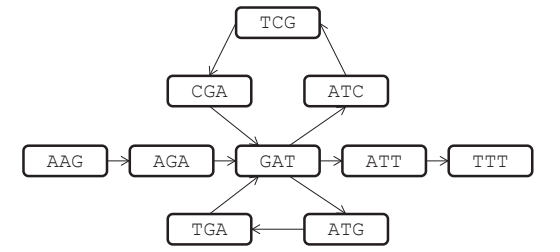
\includegraphics[width=0.7\textwidth]{Figura5_16.PNG}
\caption{De Brujinov graf $H_3$ za $R = \{AAGATC, GATCGAT, CGATGA, ATGATT, GATTT\}$ }
\label{fig:10}
\source{\cite{WingKinSung} str. 140, slika 5.16}
\end{figure}

Kao što se može videti, postoje dve Ojlerove putanje u grafu $H_3$. Ukoliko se prvo obiđe gornji ciklus, dobija se $AAGATCGATGATTT$, a ukoliko se prvo obiđe donji ciklus, dobija se $AAGATGATCGATTT$. Ovaj primer ukazuje na to da Ojlerova putanja mozda neće uvek dati ispravnu sekvencu. Čak još gore, Ojlerova putanja možda neće postojati u nekom grafu $H_k$.

U daljem tekstu govoriće se o De Brujinovom grafovskom asembleru u slučaju kada:
\begin{itemize}
    \item{ne postoji greška sekvencioniranja}
    \item{postoji greška sekvencioniranja}
\end{itemize}

\subsubsection{De Brujinov asembler (bez greške sekvencioniranja)}

Kako Ojlerova putanja nije jedinstvena i možda i ne postoji, ne teži se dobijanju kompletnog genoma. Umesto toga, teži se dobijanju skupa kontiga. Kontiga je maksimalna prosta putanja u $H_k$. Preciznije, svaka maksimalna prosta putanja je maksimalna putanja u $H_k$ tako da svaki čvor (osim početnog i krajnjeg) ima unutrašnji i spoljašnji stepen jedan. 

\begin{comment}
Slika \ref{fig:11} daje pseudokod ovog jednostavnog metoda:


%Algoritam De Brujinov asembler
%Figura 5.17
\begin{figure}[!ht]
\centering
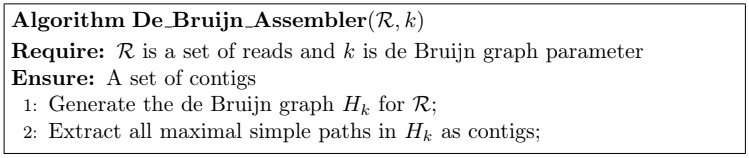
\includegraphics[width=0.9\textwidth]{Figura5_17.PNG}
\caption{Jednstavan De Brujinov grafovski asmbler}
\label{fig:11}
\source{\cite{WingKinSung} str. 141, slika 5.17}
\end{figure}

\end{comment}

Za De Brujinov graf $H_3$ sa slike \ref{fig:10} mogu se konstruisati 4 kontige: $AAGAT$, $GATCGAT$, $GATGAT$, $GATTT$. Parametar $k$ je veoma važan. Za različito $k$, mogu se dobiti različiti skupovi kontiga. Slika \ref{fig:12} ilustruje ovaj problem na De Brujinovom grafu za $k = 4$ i $k = 5$:

%Figura 5.18
\begin{figure}[!ht]
\centering
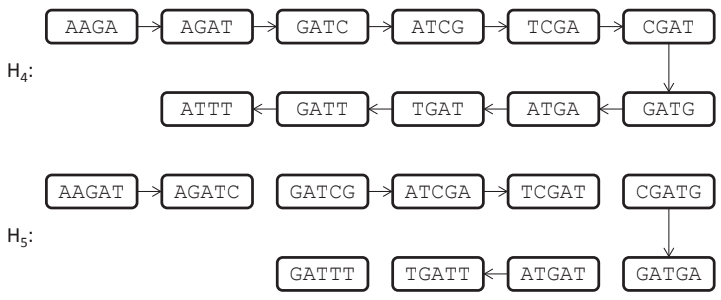
\includegraphics[width=0.9\textwidth]{Figura5_18.PNG}
\caption{De Brujinov graf $H_4$ i $H_5$ za $R = {AAGATC, GATCGAT, CGATGA, ATGATT, GATTT}$}
\label{fig:12}
\source{\cite{WingKinSung} str. 141, slika 5.18}
\end{figure}

Kada je $k = 4$, $H_4$ je prosta putanja i može se konstruisati jedna kontiga $AAGATCGATGATTT$. U slučaju da je $k = 5$, $H_5$ sadrži 5 povezanih komponenti, svaka je prosta putanja i može se konstruisati 5 kontiga: $AAGATC$, $GATCGAT$, $CGATGA$, $ATGATT$, $GATTT$.

Iz gore navedenih primera, može se primetiti da je De Brujinov graf dobar, ukoliko se zna ispravno k. Kada je k malo (pogledati $H_3$ na slici \ref{fig:10}), postoji veliki broj grana zbog ponovaka i rezultat je veliki broj kratkih kontiga. Kada je k veliko (pogledati $H_5$ na slici \ref{fig:12}), neki k-meri nedostaju. Ovo rezultuje nepovezanim komponentama, koje takođe generišu veliki broj kratkih kontiga. Tako da se mora identifikovati ispravno k kako bi se pronašla ravnoteža između ova dva problema.

\subsubsection{De Brujinov asembler (sa greškama sekvencioniranja)}

U prethodnom odeljku se pretpostavljalo da ne postoje greške sekvencioniranja u očitavanjima, što je nerealno. Kada postoje greške, pokušava se njihovo uklanjanje "čišćenjem" De Brujinovog grafa. Rešenje koje će se razmatrati su predložili Zerbino (engl. \textit{Zerbino}) i Birni (enlg. \textit{Birney}). Treba obratiti pažnju da kratka očitavanja imaju nisku stopu greške (jedna greška na svakih 100 baza), a većina k-mera sadrži najviše jednu grešku. Ovi k-meri sa greškom mogu kreirati dva moguća anomalna podgrafa u De Brujinovom grafu: \textbf{vrh (špic)} i \textbf{mehurić}.

\textbf{Vrh} je putanja dužine najviše $k$ gde svi unutrašnji čvorovi imaju ulazni i izlazni stepen 1, dok jedan od njihovih krajeva ima ulazni ili izlazni stepen 0. To može proizvesti potencijalnu kontigu dužine najviše $2k$.

%Figure 5.19
\begin{figure}[!ht]
\centering
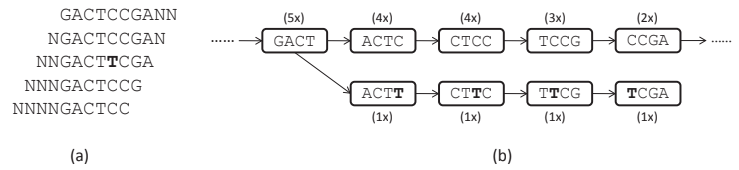
\includegraphics[width=\textwidth]{Figura5_19.PNG}
\caption{Formiranje vrha}
\label{fig:13}
\source{\cite{WingKinSung} str. 142, slika 5.19}
\end{figure}

Slika \ref{fig:13}(a) predstavlja višestruko poravnanje skupa od pet očitavanja, gde treće očitavanje ima grešku sekvencioniranja (prikazana podebljanim fontom). Slika slika \ref{fig:13}(b) predstavlja De Brujinov graf koji odgovara skupu očitavanja sa prvog dela slike i vrh koji je formiran usled jednog nepoklapanja u jednom očitavanju, tj. usled pomenute greške. Brojevi u zagradama označavaju mnogostrukost 4-mera. Ovaj vrh se može ukloniti iz De Brujinovog grafa, ali uklanjanje jednog vrha može generisati nove vrhove. Tako da procedura uklanjanja mora uklanjati vrhove rekurzivno.
% Ide pre ovaj vrh se može ukloniti Ako su svi čvorovi na vrhu %niske mnogostrukosti (k-meri koji se mali broj puta %pojavljuju u očitavanjima), takva kratka kontiga teško da %može biti ispravna (preformulisati).

\textbf{Mehurić} se sastoji od dve različite kratke putanje sa istim početnim i
krajnim čvorovima u De Brujinovom grafu, pri čemu su te dve putanje zapravo kontige koje se razlikuju u samo jednom nukleotidu. Na primer, slika \ref{fig:133}(a) sadrži skup očitavanja gde treće očitavanje ima jedno nepoklapanje. Slika \ref{fig:133}(b) prikazuje odgovarajući De Brujinov graf i jedan mehurić koji se formira. Gornja putanja mehurića predstavlja $GACTCCGAG$, dok donja putanja predstavlja $GACTTCGAG$. Kada su dve putanje u mehuriću veoma slične, putanja sa nižom mnogostukošću će verovatno biti lažno pozitivna. Može se pokušati sa spajanjem (otklanjanjem) mehurića. U ovom primeru, 2 putanje imaju samo jedno nepoklapanje. Budući da su čvorovi u donjoj putanji niže mnogostrukosti, vrši se spajanje (otklanjanje) mehurića i dobija se graf na slici \ref{fig:13}(c). Preciznije, može se definisati \textbf{težina putanje} $w_1 \rightarrow w_2 \rightarrow ... \rightarrow w_p$ kao $\sum_{i=1}^{p} f(w_i)$, gde je $f(w_i)$ mnogostrukost od $w_i$. Onda, kada se dve putanje spoje u mehuriću, zadržava se ona sa većom težinom.

%Figure 5.20
\begin{figure}[!ht]
\centering
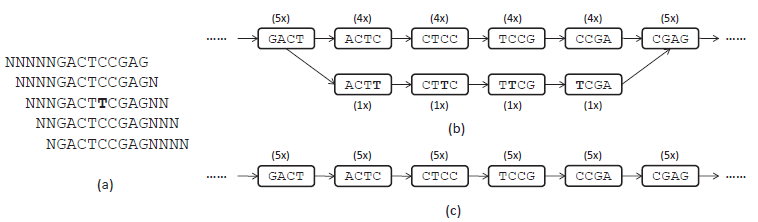
\includegraphics[width=\textwidth]{Figura5_20.PNG}
\caption{Formiranje mehurića}
\label{fig:133}
\source{\cite{WingKinSung} str. 143, slika 5.20}
\end{figure}

Za spajanje (otklanjanje) mehurića, može se koristiti \textbf{algoritam turneje} (engl. \textit{tour bus algorithm}). Ovaj algoritam je nalik na Dijkstrinu pretragu u širinu baziranu na \textit{BFS} metodu. Algoritam počinje od proizvoljnog čvora $s$ i posećuje čvorove u rastućem poretku rastojanja od početnog čvora. Kada algoritam obrađuje neposećeni čvor $u$, on proverava i svako njegovo dete $v$. Za svako $v$ se izvode dva koraka. Prvo, dodeljuje se $u$ kao roditelj od $v$ u $BFS$ stablu postavljanjem $\pi (v) = u$. Drugo, ako je dete $v$ od $u$ posećeno, mehurić je detektovan. Algoritam izračunava najnižeg zajedničkog pretka $c$ od $u$ i $v$ u $BFS$ stablu definisanog sa $\pi ()$. Zatim se putanje $c \rightarrow u$ i $c \rightarrow v$ upoređuju. Ako su dovoljno slične, spajaju se. Zadržavamo putanju sa većom težinom.

\begin{comment}

Algoritam je detaljnije prikazan na slici \ref{fig:14}:

\newpage

%Figure 5.21
\begin{figure}[!ht]
\centering
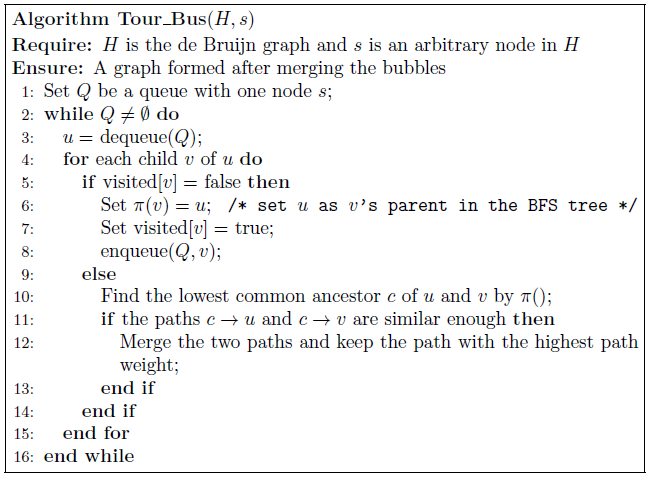
\includegraphics[width=0.8\textwidth]{Figura5_21.PNG}
\caption{Algoritam turneje}
\label{fig:14}
\source{\cite{WingKinSung} str. 144, slika 5.21}
\end{figure}


Slika \ref{fig:15} ilustruje korake algoritma turneje. Originalni De Brujinov graf je prikazan na slici \ref{fig:15}(a). Počevši od čvora $r$, \textit{BFS traversal} se izvodi kako bi se posetili svi potomci od $r$ u rastućem poretku rastojanja od $r$. \textit{BFS traversal} se zaustavlja kada dođe do posećivanja već posećenog čvora. Slika \ref{fig:15}(b) prikazuje BFS stablo (podebljano) kada je čvor $v$ ponovo posećen od strane čvora $u$. Identifikovanjem najnižeg zajedničkog pretka $c$ u BFS stablu, pronalaze se 2 putanje $c \rightarrow u$ i $c \rightarrow v$ koje formiraju mehurić. Vrši se spajanje 2 putanje i zadržava se putanja sa većom težinom. Nakon formiranja mehurića, dobija se slika \ref{fig:15}(c). Zatim se BFS nastavlja. Nakon što BFS poseti $u'$, ponovo posećuje $v'$. $c'$ je najniži zajednički predak od $u'$ i $v'$. Pronalaze se 2 putanje $c' \rightarrow u'$ i $c' \rightarrow v'$ koje formiraju mehurić. Nakon otklanjanja mehurića, dobija se slika \ref{fig:15}(d). Zatim, ne može se pronaći više nijedan mehurić i algoritam turneje se završava.

\newpage

%Figure 5.22
\begin{figure}[!ht]
\centering
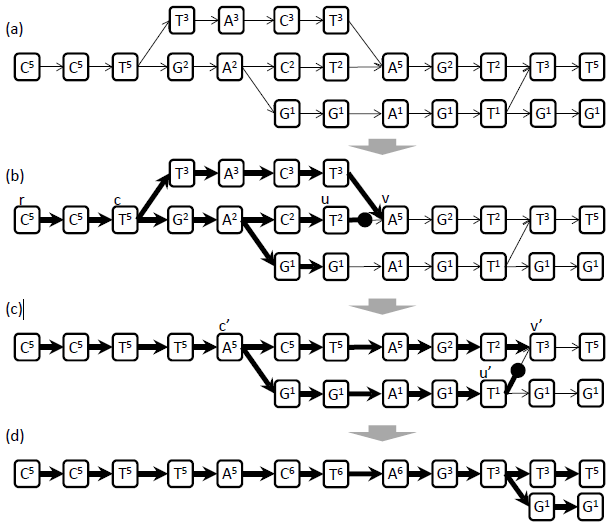
\includegraphics[width=0.8\textwidth]{Figura5_22.PNG}
\caption{Ovaj primer ilustruje kako algoritam turneje obilazi De Brujinov graf. Radi jasnoće, svaki čvor pokazuje poslednju bazu svojih k-mera i odgovarajući celobrojni stepen je njegova mnogostrukost. Algoritam izvodi pretragu u dobinu (BFS) i BFS stablo je prikazano podebljanim ivicama. Na slici (a) postoje 2 (ugnježdena) mehurića. Na slici (b) se izvodi BFS počevši od $r$. Kada se poseti $u$, dete $v$ od $u$ je posećeno. Identifikuje se mehurić i vrši se njegovo spajanje. Zatim, dobija se slika (c). Na slici (c) se nastavlja izvođenje BFS algoritma. Kada se posete $u'$, dete $v'$ od $u'$ je posećeno. Identifikuje se drugi mehurić i vrši se njegovo spajanje. Zatim se dobija slika (d). Na slici (d) se nastavlja izvođenje BFS algoritma. Kako se ne može identifikovati više nijedan mehurić, algoritam se završava.}
\label{fig:15}
\source{\cite{WingKinSung} str. 145, slika 5.22}
\end{figure}

\end{comment}

Nakon što se uklone vrhovi i spoje (otklone) mehurići u De Brujinovom grafu, može se dalje filtrirati buka uklanjanjem k-mera sa mnogostrukošću manjom ili jednakom nekom pragu. Na primer na slici \ref{fig:15}(d), ako je $m = 1$, treba ukloniti dve ivice težine 1. Ova tehnika se takođe koristi pri korigovanju grešaka u sekvencioniranju. Ukratko, predstavljena su 3 trika: (1) otklanjanje vrhova, (2) spajanje mehurića i (3) filtriranje k-mera sa niskom mnogostrukošću. Kombinovanjem ovih tehnika, dobija se algoritam koji može da obradi greške sekvencioniranja i prikazan je na slici \ref{fig:16}:

%Figure 5.23
\begin{figure}[!ht]
\centering
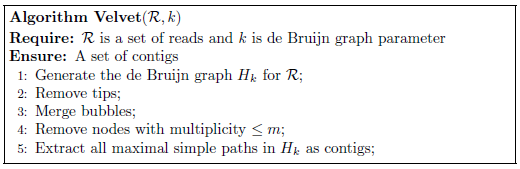
\includegraphics[width=0.9\textwidth]{Figura5_23.PNG}
\caption{Algoritam za otklanjanje grešaka sekvencioniranja}
\label{fig:16}
\source{\cite{WingKinSung} str. 146, slika 5.23}
\end{figure}

\newpage

\subsection{Kako izabrati k?}

Kao što je već rečeno, odabir broja $k$ može uticati na performanse De Brujinovog algoritma. Jednostavno rešenje je pokretanje algoritma sa slike \ref{fig:16} za različite $k$. Zatim se kontige grupišu i spajaju. Jedan od problema sa ovim jednostavnim rešenjem je što kontige dobijene za različito $k$ imaju različit kvalitet. Kontige dobijene od $H_k$ gde je $k$ malo su veoma tačne. Međutim, takve kontige su kratke, jer postoji veliki broj grana zbog ponovaka. Kontige dobijene od $H_k$ gde je $k$ veliko su duže. Međutim, one mogu sadržati mnogo grešaka.

IDBA asembler\footnote{IDBA - \textit{A Practical Iterative de Bruijn Graph De Novo Assembler}} počiva na ideji da ne traba graditi De Brujinov graf nezavisno za različite $k$. Umesto toga, IDBA gradi De Brujinov graf $H_k$ postepeno krećući od malih $k$ i idući ka većim. Kada je $k$ malo, mogu se dobiti visokokvalitetne kontige, iako su kratke. Zatim se ove kontige koriste za ispravljanje grešaka u očitavanjima. Postepeno se izgrađuje De Brujinov graf $H_k$ za sve veće $k$. Kako su očitavanja u $R$ korigovana, buka u $H_k$ je redukovana. Na ovaj način se za veliko $k$ omogućava dobijanje dugih kontiga visokog kvaliteta iz $H_k$.

\begin{comment}
Slika \ref{fig:17} opisuje ideju IDBA asemblera:

%Figure 5.24
\begin{figure}[!ht]
\centering
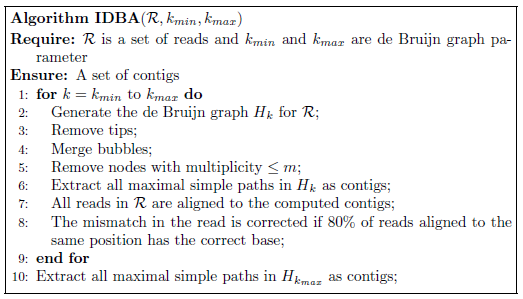
\includegraphics[width=0.9\textwidth]{Figura5_24.PNG}
\caption{IDBA}
\label{fig:17}
\source{\cite{WingKinSung} str. 146, slika 5.24}
\end{figure}

\end{comment}

\chapter{Opis implementacije algoritama i rezultati njihovog izvršavanja}

U prethodnom delu data je biološka osnova za algoritme koji se primenjuju u sekvencioniranju genoma. U ovom delu će biti dati opisi implementacije tih algoritama u programskom jeziku Elixir, kao i delovi koda radi boljeg razumevanja. Svaki algoritam je definisan u okviru modula koji nosi naziv tog algoritma i koji sadrži glavnu funkciju i veliki broj pomoćnih.

\section{Opis JellyFish algoritma}

Ulaz u glavnu funkciju:

\begin{itemize}
    \item {$Z$ je skup od $N$ k-mera, koji je u Elixir-u predstavljen listom stringova}
    \item {$\alpha$ je faktor opterećenja koji kontroliše veličinu heš tabele i koji je broj tipa float između 0 i 1}
    \item {h je heš funkcija koja k-mere, tj. stringove mapira u brojeve}
\end{itemize}

\newpage

Heš funkcija koja nosi naziv \textit{pattern\_to\_number} prikazana je na listingu \ref{lst:100}:

\lstinputlisting[language=erlang,label={lst:100},caption=Heš funkcija \textit{pattern\_to\_number},captionpos=b]{101.ex}

Argumenti funkcije su string koji predstavlja k-mer (\textit{pattern}), početni string koji je uvek prazan pri pozivu funkcije (\textit{begin\_string}), indeks  koji je uvek 0 pri pozivu funkcije (\textit{index}) i dužina k-mera (\textit{length\_of\_pattern}). Ova funkcija je rekurzivna i poziva se za svaki karakter stringa \textit{pattern}, počevši od nulte pozicije, sve dok se ne prođe kroz ceo string, tj. dok se \textit{index} ne izjednači sa \textit{length\_of\_pattern}. Dakle, uzima se prvi karakter \textit{pattern}-a, kodira se pomoćnom funkcijom \textit{symbol\_to\_number}, prikazanom na listingu \ref{lst:101} i nadovezuje se na \textit{begin\_string} pomoću operatora za nadovezivanje stringova $<>$. Zatim se prelazi na sledeći karakter, ponavlja se postupak i sve tako dok se ne dođe do kraja \textit{pattern}-a. U tom trenutku, povratna vrednost funkcije je \textit{begin\_string} koji umesto $A$, $C$, $G$ i $T$ sadrži kodove $00$, $01$, $10$, $11$, respektivno i koji se pomoću funkcije \textit{to\_integer/2} iz modula \textbf{String} pretvara u ceo broj.

\lstinputlisting[language=erlang,label={lst:101},caption=Pomoćna funkcija \textit{symbol\_to\_number},captionpos=b]{100.ex}

Glavna funkcija pre poziva pomoćnih funkcija obavlja početnu inicijalizaciju objekata koji su joj potrebni, tj. izračunava veličinu heš table $H$ i $Count$ tabele, a zatim ih inicijalizuje praznim stringovima i nulama, respektivno. Izgled glavne funkcije može se videti na listingu \ref{lst:102}:

\newpage

\lstinputlisting[language=erlang,label={lst:102},caption=Glavna funkcija \textit{jellyfish\_algorithm},captionpos=b]{102.ex}

Funkcije za inicijalizaciju H tabele (\textit{build\_h\_table}) i Count tabele (\textit{build\_count\_table}), a koje su predstavljene mapama $h\_table$ i $count\_table$, identične su i imaju iste ulazne parametre. Jedina razlika je što su vredosti mape $h\_table$ na početku prazni stringovi, a mape $count\_table$ nule, što se može videti na listingu \ref{lst:103}:

\lstinputlisting[language=erlang,label={lst:103},caption=Funkcije za inicijalizaciju H i Count tabela,captionpos=b]{103.ex}

Pomoćna funkcija koja obavlja brojanje k-mera je funkcija \textit{calculate} čiji su argumenti mape \textit{h\_table} i \textit{count\_table}, lista \textit{z\_table} i veličina pomenutih mapa \textit{size\_of\_H}. Kod ove funkcije prikazan je na listingu \ref{lst:104}: 

\newpage

\lstinputlisting[language=erlang,label={lst:104},caption=Pomoćna funkcija \textit{calculate},captionpos=b]{104.ex}

Kao što se može videti, funkcija \textit{calculate} je rekurzivna. Poziva se za svaki element liste \textit{z\_table}, počevši od njene glave, sve dok lista ne postane prazna. Za svaki string iz \textit{z\_table} prvo se poziva funkcija \textit{hashEntry} koja vrši heširanje stringova u indeks \textit{i} koji ključ za mape \textit{h\_table} i \textit{count\_table}. Kod ove funkcije dat je listingom \ref{lst:105}:

\lstinputlisting[language=erlang,label={lst:105},caption=Pomoćna funkcija \textit{hashEntry},captionpos=b]{105.ex}

Zatim se proverava da li je vredost ključa \textit{i} u mapi \textit{h\_table} prazan string. Vrednost ključa neke mape se u Elixir-u dohvata pomoću funkcije \textit{get/2} iz modula \textbf{Map} čiji su argumenti naziv mape i ključ. Ukoliko je vrednost prazan string, ključu se dodeljuje vrednost stringa koji se trenutno obrađuje i ključu u mapi \textit{count\_table} \textit{i} se dodeljuje vrednost 1. Vrednost ključa nekoj mapi se dodeljuje pomoću funkcije \textit{put/3} pomenutog modula. Njeni argumenti su naziv mape, ključ i vrednost koja se dodeljuje. Ako je vrednost ključa \textit{i} u mapi \textit{h\_table} različita od praznog stringa, onda se samo vrednost ključa \textit{i} u mapi \textit{count\_table}  povećava za jedan i prelazi se na obradu sledećeg stringa iz liste \textit{z\_table}. 

Na kraju, izlaz iz glavne funkcije je uređeni par $(\textit{h\_table}, \textit{count\_table})$. Kao što je već pomenuto, u Elixir-u su predstavljeni mapama veličine koja je količnik dužine liste \textit{z\_table} i faktora opterećenja \textit{alpha}. Obe mape imaju iste ključeve, dok su im vrednosti stringovi koji predstavljaju k-mere i brojevi koji predstavljaju broj pojavljivanja određenog stringa u listi \textit{z\_table}.

Na listingu \ref{lst:105} se može videti konkretan primer pokretanja algoritma:

\lstinputlisting[language=erlang,label={lst:106},caption=Primer pokretanja \textit{JellyFish} algoritma,captionpos=b]{jellyfish_pokretanje.ex}

\newpage

Ovo je primer izvršavanja algoritma u komandnom promptu. Za kompajliranje fajla u kome se nalazi algoritam i pokretanje interaktivnog Elixir-a, navodi se komanda \textit{iex jellyfish.ex}. Nakon toga mogu se pozivati funkcije tako što se prvo navede ime modula u okviru koga su definisane, tačka, pa naziv funkcije i njeni argumenti. U ovom slučaju to su modul \textit{JellyFish}, funkcija \textit{jellyfish\_algorithm}, lista stringova $["AC", "CG", "AC", "GT", "CA","GG", "AC","GT"]$ koji predstavljaju k-mere i faktor opterećenja 0.7.


% ------------------------------------------------------------------------------
\chapter{Zaključak}
% ------------------------------------------------------------------------------
%\pangrami

%\pangrami

% ------------------------------------------------------------------------------
% Literatura
% ------------------------------------------------------------------------------
\literatura

% ==============================================================================
% Završni deo teze i prilozi
\backmatter
% ==============================================================================

% ------------------------------------------------------------------------------
% Biografija kandidata
\begin{biografija}
  \textbf{Vuk Stefanović Karadžić} (\emph{Tršić,
    26. oktobar/6. novembar 1787. — Beč, 7. februar 1864.}) bio je
  srpski filolog, reformator srpskog jezika, sakupljač narodnih
  umotvorina i pisac prvog rečnika srpskog jezika.  Vuk je
  najznačajnija ličnost srpske književnosti prve polovine XIX
  veka. Stekao je i nekoliko počasnih mastera.  Učestvovao je u
  Prvom srpskom ustanku kao pisar i činovnik u Negotinskoj krajini, a
  nakon sloma ustanka preselio se u Beč, 1813. godine. Tu je upoznao
  Jerneja Kopitara, cenzora slovenskih knjiga, na čiji je podsticaj
  krenuo u prikupljanje srpskih narodnih pesama, reformu ćirilice i
  borbu za uvođenje narodnog jezika u srpsku književnost. Vukovim
  reformama u srpski jezik je uveden fonetski pravopis, a srpski jezik
  je potisnuo slavenosrpski jezik koji je u to vreme bio jezik
  obrazovanih ljudi. Tako se kao najvažnije godine Vukove reforme
  ističu 1818., 1836., 1839., 1847. i 1852.
\end{biografija}
% ------------------------------------------------------------------------------

\end{document}